\documentclass[anon,12pt]{colt2026} % Anonymized submission
%\documentclass[final,12pt]{colt2026} % Include author names

% The following packages will be automatically loaded:
% amsmath, amssymb, natbib, graphicx, url, algorithm2e

\usepackage{indentfirst}
\usepackage{tikz}
\usetikzlibrary{shapes.geometric, arrows, positioning}
\usepackage{caption}
\usepackage{algorithm2e}

% Configure algorithm2e style
\SetAlFnt{\small}
\SetAlCapFnt{\normalsize}
\SetAlCapNameFnt{\normalsize}
\SetNlSty{textbf}{}{}

\newcommand{\br}[1]{\mathopen{}\left( #1 \right)}
\newcommand{\brc}[1]{\mathopen{}\left\{ #1 \right\}}
\newcommand{\spr}[1]{\mathopen{}\left| #1 \right|}
\newcommand{\fl}[1]{\mathopen{}\left\lfloor #1 \right\rfloor}
\newcommand{\cl}[1]{\mathopen{}\left\lceil #1 \right\rceil}
\newcommand{\angl}[1]{\mathopen{}\langle #1 \rangle}
\newcommand{\e}[1]{\exp\left\{ #1 \right\}}

\newcommand{\ecc}{\operatorname{ecc}}
\newcommand{\rad}{\operatorname{rad}}
\newcommand{\diam}{\operatorname{diam}}
\newcommand{\Rim}{\operatorname{Rim}}
\newcommand{\rim}{\operatorname{rim}}
\newcommand{\Anc}{\operatorname{Anc}}
\newcommand{\cov}{\operatorname{cov}}

\newcommand{\NPcomplete}{\textnormal{$\mathcal{NP}$-Complete}}
\newcommand{\NPhard}{\textnormal{$\mathcal{NP}$-Hard}}
\newcommand{\polyAPXcomplete}{\textnormal{Poly–$\mathcal{APX}$–Complete}}

\newcommand{\Cent}{\texttt{Cent}}
\newcommand{\APP}{\texttt{APP}}
\newcommand{\OPT}{\texttt{OPT}}
\newcommand{\COST}{\texttt{COST}}
\newcommand{\LB}{\mathcal{LB}}
\newcommand{\HB}{\mathcal{HB}}
\newcommand{\THB}{\mathcal{THB}}
\newcommand{\THH}{\texttt{TH}}

\newcommand{\argmin}{\mathopen{}\operatorname*{arg\,min}}
\newcommand{\argmax}{\mathopen{}\operatorname*{arg\,max}}

% Theorem environments
\newtheorem{observation}{Observation}


\title[Active Learning and Covering Problems with Precedence]{Active Learning and Covering Problems with Precedence}
\usepackage{times}
% Use \Name{Author Name} to specify the name.
% If the surname contains spaces, enclose the surname
% in braces, e.g. \Name{John {Smith Jones}} similarly
% if the name has a "von" part, e.g \Name{Jane {de Winter}}.
% If the first letter in the forenames is a diacritic
% enclose the diacritic in braces, e.g. \Name{{\'E}louise Smith}

% Two authors with the same address
% \coltauthor{\Name{Author Name1} \Email{abc@sample.com}\and
%  \Name{Author Name2} \Email{xyz@sample.com}\\
%  \addr Address}

% Three or more authors with the same address:
% \coltauthor{\Name{Author Name1} \Email{an1@sample.com}\\
%  \Name{Author Name2} \Email{an2@sample.com}\\
%  \Name{Author Name3} \Email{an3@sample.com}\\
%  \addr Address}

% Authors with different addresses:
\coltauthor{%
 \Name{Michał Szyfelbein} \Email{abc@sample.com}\\
 \addr Address 1
 \AND
 \Name{Dariusz Dereniowski} \Email{xyz@sample.com}\\
 \addr Address 2%
 \AND
 \Name{Tytus Pikies} \Email{xyz@sample.com}\\
 \addr Address 3%
}

\begin{document}

\maketitle

\begin{abstract}%

  In the Bayesian Active Learning a hidden hypothesis is required to be uncovered. To do so, the learner is allowed to perform tests, each of which reveals partial information about the hidden hypothesis. Upon receiving this information, the learner adaptively selects the next test to be performed. The goal is to uncover the hidden hypothesis while performing as few tests as possible in the worst or average case. 

  In the covering problems, we are given a set of items and a collection of subsets that cover these items. The objective is to select a sequence of subsets that covers all items, which minimizing the worst or average covering cost.

  For both types of problems, a natural constraint may arise that some tests can only be performed only after certain other tests (or some subsets can only be selected after selecting certain other subsets). We model such constraints using directed acyclic graphs (DAGs) that impose precedence on the tests or subsets. 
  This paper explores the connection of active learning and covering problems under such constraints. 
  
  We show that given any bicriteria $\br{O\br{1}, \alpha}$-approximation ratio for the Precedence Constrained Set Cover, we can obtain an $O\br{\alpha\cdot \log n}$-approximation ratio for the Worst Case Active Learning with precedence constraints, where $n$ is the number of hypothesis. Similarly, we prove that given any $O\br{\beta}$-approximation ratio for the Precedence Constrained Min-Sum Set Cover, we can obtain an $O\br{\beta\cdot \log n}$-approximation ratio for the Average Case Active Learning with Precedence Constraints. Finally, we provide several approximation algorithms for the Set Cover and Min-Sum Set Cover problems with various types of precedence constraints.
\end{abstract}

\begin{keywords}%
  Bayesian active learning, Set cover, Precedence constraints, Approximation Algorithms, Decision Trees%
\end{keywords}

\section{Introduction}

Consider a set $\cH$ of $n$ \emph{hypotheses}, a set $\cT$ of $m$ \emph{tests} and  an unknown \emph{target hypothesis} $\target\in\cH$ that needs to be discovered through testing.
Each test $t\in\cT$ is a partition of $\cH$, that is, $t$ consists of subsets of $\cH$ such that $x\cap y=\emptyset$ for any $x,y\in t$ and $\bigcup_{x\in t} x=\cH$.
As a result of executing a test $t\in\cT$, \questioner recives a \emph{reply} that reveals $x\in t$ such that $\target\in x$.
That is, the \questioner learns which subset of $\cH$ that belongs to $t$ contains the target.
Each subsequent test is selected by \questioner by taking into acocunt replies from all tests to date.
Without formally stating an optimization criterion we refer to the above as the \emph{Optimal Decision Tree} ($\ProblemDT$) problem.
The goal of \questioner is to output $\target$ while minimizing either the number of tests done in the worst case or on average.
(For formal statemets of our problems see the next section).

We note that the above statement generalizes the classical binary search in (fully or partially) sorted data.
In this work we generalize this proces by considering precedence relation between tests given as an arbitrary partial order $(\cT,\preceq)$.
Then, a test $t$ can be performed only when all its predecesors had to be performed previously (to which we refer as \emph{precedence-closed} solution).
On the applicability side, the binary search itself includes numerous use cases, some of them in the area of biology \cite{BayesianLearnerOptimalNoisyBinarySearch}.
For example, if hypotheses were to represent possible conditions or deseases, and each test distinguishes between some pairs of hypotheses, then precedence constaints would represent some ordering on performing tests.
These may be enforced e.g. by cost measures (like executing several `cheaper' tests whose outcome may eliminate the need of executing a more expensive one), or by an expert.

The method to address the optimal decision tree problems is through a series of `reductions' between other optimization problems.
By this we mean an approach, where a particular algorithm for one problem implies existence of an algorithm for the other.
Particularly, we study a set cover problem with precedences:
We are given a set $\cU$ of $n$ items, a collection $\cS$ of $m$ subsets of $\cU$, such that $\bigcup_{S\in\cS}S=\cU$, an arbitrary partial order $(\cS,\preceq)$ on these subsets and an integer $k$.
We say that a subfamily $\cC\subseteq\cS$ \emph{covers} at least $k$ items from $\cU$ if $\spr{\bigcup_{C\in\cC}C}\geq k$.
We ask for a $\cC\subseteq\cS$ that covers at least $k$ items from $\cU$ and is \emph{precedence-closed}, that is, for each $x\in\cC$ and each $y\in\cS$ such that $y\preceq x$ it holds $y\in\cC$.
The approximation algorithms that we propose en route, e.g. for precedence constrained set cover, are of independent interest.

% \medskip
% \paraTitle{Outline.}
% In the next section we formally state all problems we address in this work.
% Section~\ref{sec:our-results} gives an overview of the main results of this work.
% Section~\ref{sec:AL} provides approximation algorithm for the above decision tree problem, assuming there exist certain approximations for variants of set cover.
% The latter are developed in Section~\ref{sec:SC}.
% Finally, set cover is solved via dense subfamily approximation from Section~\ref{sec:MDPCS}.
% The algorithms are supplemented with a number of inapproximability results in Section~\ref{sec:hardness}.

% Consider following problems:
% \begin{itemize}
%   \item  The \emph{Precedence Constrained Bayesian Decision Tree Problem} consists a set of $\mathcal{H}$ of $n$ hypothesis, a set $\cT$ of $m$ tests and a DAG (directed acyclic graph) $\mathcal{F} = \brc{\cT, \preceq}$ encoding the precedence constraints between available tests. Among $\mathcal{H}$ a hidden hypothesis is required to be encovered. To do so, the learner is allowed to perform tests, each of which reveals partial information about the hidden hypothesis. Upon receiving this information, the learner actively selects the next test to be performed. Importantly, in order to perform such test the learner needs to perform all of its predecesors in $\mathcal{F}$ first. The goal is to uncover the hidden hypothesis while performing as few tests as possible. Depending on the chosen criterion we distinguish between the \emph{Precedence Constrained Worst Case Decision Tree} (PCWCDT) and \emph{Precedence Constrained Average Case Decision Tree} (PCACDT) problems.
%   \item The \emph{Precedence Constrained Covering Problem} consists of a set of $n$ items $\mathcal{U}$, a collection $\mathcal{S}$ of $m$ subsets of $\mathcal{U}$ that cover these items, and a DAG $\mathcal{F} = \brc{\mathcal{S}, \preceq}$ encoding the precedence constraints between available subsets. The goal is to select a sequence of tests that covers at least $K$ items. Depending on the chosen criterion we distinguish between the \emph{Precedence Constrained Set Cover} (PCSC) and \emph{Precedence Constrained Min-Sum Set Cover} (PCMSSC) problems. In the first we are only interested in minimizing the number of selected subsets, while in the second we want to minimize the average time it takes to cover an item.
% \end{itemize}

\subsection{Problem formulations and outline} \label{sec:problems}

\DD{ta sekcja jest w miare ulozona pod ustalenia na discord; z wyjatkiem dwoch ostatnich problemow -- do decyzji czy potrzebne}

After introducing necessary notation in Section~\ref{sec:preliminaries}, we provide algorithms (cf. Section~\ref{sec:AL}) for the decision tree problems.
\begin{problem}[Precedence Constrained Worst Case Decision Tree ($\ProblemPCWCDT$)] \label{problem:PCWCDT}
Given a set of hypotheses $\cH$, a set of tests $\cT$ and a precedence relation $(\cT,\preceq)$ on tests, find a precedence-closed decision tree strategy that outputs the target hypothesis by performing the minimum number of tests in the worst case.
\end{problem}
\begin{problem}[Precedence Constrained Average Case Decision Tree ($\ProblemPCACDT$)] \label{problem:PCACDT}
Given a set of hypotheses $\cH$, a set of tests $\cT$ and a precedence relation $(\cT,\preceq)$ on tests, find a precedence-closed decision tree strategy that outputs the target hypothesis $\target$ and minimizes the sum $\sum_{h\in\cH}c(h)$, where $c(h)$ is the number of tests performed when $h=\target$.
\end{problem}
Whenever the criterion is not important or we want to make a claim that applies both to $\ProblemPCWCDT$ and $\ProblemPCACDT$, we use the symbol $\ProblemPCDT$ to refer to a \emph{Precedence Constrained Decision Tree} instance.

The algorithms for the above are conditioned on existence of approximations for the set cover.
These in turn are obtained via a reduction from a problem of finding a maximum density subset (cf. Section~\ref{sec:MDPCS}).
The \emph{density} $\Delta$ of a nonempty subfamily $\cA$ on a universum $X$ ($A\subseteq X$ for each $A\in\cA$) is
\[
\Delta\br{\cA, X} \equiv \frac{\spr{\cov\br{\cA, X}}}{\spr{\cA}}
\]
For convenience, we define $\Delta\br{\emptyset, X} < 0$.
We also write $\Delta\br{\cA}$ when $X$ is the universum.
\begin{problem}[Max-Density Precedence-Closed Subfamily ($\ProblemMDPCS$)]
Given a universum $\cU$ of $n$ items, a family $\cG$ of $m$ subsets of $\cU$ and a precedence relation $(\cG,\preceq)$, find a precedence-closed subfamily $\cA \subseteq \mathcal{G}$ that maximizes $\Delta\br{\cA}$.
\end{problem}
We will also need a `bounded' version:
\begin{problem}[Bounded Max-Density Precedence-Closed Subfamily ($\ProblemBMDPCS$)]
Given a universum $\cU$ of $n$ items, a family $\cG$ of $m$ subsets of $\cU$, a precedence relation $(\cG,\preceq)$ and an integer $B>0$, find a precedence-closed subfamily $\cA \subseteq \mathcal{G}$ that maximizes $\Delta\br{\cA}$ and $\spr{\cA}\leq B$.
\end{problem}

Having proved the necessary claims on $\ProblemMDPCS$ and $\ProblemBMDPCS$, we develop in Section~\ref{sec:SC} the algorithms for set cover variants introduced below.
For any partial order $(X,\preceq)$ and $S\subseteq X$ let $\closure{S}$ denote the minimal precedence-closed subset of $X$.
For a family of sets $\cA$ its \emph{coverage} is $\cov\br{\cA}=\bigcup_{A\in\cA}A$, and by extension, $\cov\br{\cA, X} = \cov\br{\cA} \cap X$ for any set $X$.
\begin{problem}[Precedence Constrained Set Cover ($\ProblemPCSC$)]
Given a universum $\cU$ of $n$ items, a family $\cS$ of $m$ subsets of $\cU$, a precedence relation $(\cS,\preceq)$ and $0<f<1$, find a precedence-closed subfamily $\cC\subseteq\cS$ that covers at least $fn$ items and minimizes $\spr{\cC}$.
\end{problem}
A permutation $\br{C_1,\ldots,C_l}$ of the elements in $\cC$ is \emph{consistent} with the partial order $(\cS,\preceq)$ if for any $C_i$ and $C_j$ such that $C_i\preceq C_j$ it holds $i<j$.
The \emph{coverage time} of a $x\in\cov\br{\cC}$ is the minimum index $i$ such that $x\in C_i$.
\begin{problem}[Precedence Constrained Min-Sum Set Cover ($\ProblemPCMSSC$)]
Given a universum $\cU$ of $n$ items, a family $\cS$ of $m$ subsets of $\cU$, a precedence relation $(\cS,\preceq)$ and $0<f<1$, find a precedence-closed sequence $(C_1,\ldots,C_l)$ that covers at least $fn$ items and minimizes the sum of coverage times of the elements in $C_1\cup\cdots\cup C_l$.
\end{problem}
\begin{problem}[Budgeted Precedence Constrained Set Cover ($\ProblemBPCSC$)]
Given a universum $\cU$ of items, a family $\cS$ of subsets of $\cU$ and a budget $B>0$, find a precedence-closed set cover $\cC$ that maximises the number of covered items and satisfies $\spr{\cC}\leq B$.
\end{problem}

Our results are supplemented with a number of inapproximability results in Section~\ref{sec:hardness}.


\DD{A te dwa problemy to na razie resztowka, ktora gdzies powinna trafic}
\begin{problem}[Group Steiner Tree (GST)]
Given an undirected graph $G = (V, E)$ with edge costs, a root vertex $r \in V$, and groups $g_1, \ldots, g_k \subseteq V$, find a minimum-cost tree $T$ rooted at $r$ that contains at least one vertex from each group $g_i$.
\end{problem}

\begin{conjecture}[Planted Dense Subgraph (PDS) Conjecture]
For any constants $\beta < \alpha$ and any $k\geq \sqrt{N}$, there is no polynomial time algorithm that can distinguish between the following two distributions of graphs with any advantage $\epsilon > 0$: (1) With probability 1/2, an Erdős-Renyi graph $G(N, N^{\alpha - 1})$, (2) With probability 1/2, an Erdős-Renyi graph $G(N, N^{\alpha - 1})$ with a planted subgraph of size $k$ and edge density $k^{\beta - 1}$.
\end{conjecture}

\begin{problem}[Precedence constrained test cover (PCTC)]
Given a set $\cH$ of $n$ hypotheses, a set $\cT$ of $m$ tests, and a partial order $\brc{\cT, \preceq}$ encoding precedence constraints for $\cT$, find a precedence-closed subfamily of tests that distinguishes all pairs of hypotheses.
\end{problem}


\subsection{Related Work}

\paragraph{Optimal Decision Tree}
Optimal decision tree is among the classical problems in computer science and has been studied extensively, starting with Garey \cite{GareyPerfBoundsOnSplittingAlgForBinTesting} in the 1970s. 
Since that time, it has gathered a lot of attention due to its numerous applications which include medical diagnosis, troubleshooting, active learning, and information retrieval. 
This problem is usually studied under two different optimization criteria: minimizing the worst-case cost and minimizing the average-case cost. 
Both versions of the problem are known to be NP-hard and cannot be approximated within an $o\br{\log n}$ factor \cite{ConstructOptimalBinaryDecisionTreesIsNPComplete,HardnessOfMinHeightDTP,ApproximatingDecisionTreesMultiwayBranches,DiagnosisDetermination}. Moreover, this bound is known to be tight and several $\cO(\log n)$-approximation algorithms for both non-uniform probabilities and cost average-case \cite{OptimalSplitTreeProblem,AnalysisGreedyActiveLearning,ApproximatingDecisionTreesMultiwayBranches,AverageCaseActiveLearningWithCosts,ApproximatingOptimalBinaryDecisionTrees,DTsforEntIdent,ApproxAlgsForOptDTsAndAdapTSPProblems,DiagnosisDetermination,AdaptiveSubmodularRankingAndRouting,AdaptivityInAdaptiveSubmodularity,MinimumCostAdaptiveSubmodularCover} as well as worst case \cite{DecisionTreesForGeometricModels,TheCostComplexityOfInteractiveLearning,DiagnosisDetermination}. Despite the hardness of the problem several special cases are known to have $o\br{\log n}$-approximation algorithms. For average case, this includes when tests have a constant number of possible outcomes and all probabilities and costs are uniform an $\cO\br{\log n/\log \log n}$-approximation is known \cite{TightAnalysisGreedyUniformDecisionTree}. This variant cannot be approximated within $\br{4-\epsilon}$ factor for any $\epsilon > 0$ unless P = NP \cite{DTsforEntIdent}. Moreover achieving any approximation factor above $9$ is not NP-hard assuming ETH \cite{TightAnalysisGreedyUniformDecisionTree}.
For worst case, when the underlying search space is a partially ordered set with a maximum element and costs are uniform an $\cO\br{\log n/\log \log n}$-approximation is known \cite{EdgeRankingSearchingPartialOrders}.


\paragraph{Searching in Trees}
For a special case when the instance represents searching in a tree, i.e., the set of hypothesis represents vertices of a tree and tests inform about the direction of the target placement with respect to the queried element (depending on the model, either vertices or edges can be queried), the problem has also been extensively studied. For uniform costs and worst-case criterion, a linear time exact algorithm is known for both edge query and vertex query variant \cite{Schaffer1989OptNodeRankOfTsInLinTime,OnakParys2006GenOfBSSInTsAndFLikePosets,Mozes_Onak2008FindOptTSStartInLinTime}. For average case, uniform costs and vertex queries an FPTAS is known \cite{SearchTreesOnGraphs}. For edge queries the problem is known to be NP-hard \cite{OnTheComplexityOfSearchingInTreesAverageCaseMinimization} and a greedy strategy achieves $3/2$-approximation \cite{TightApproximationBoundsOnASimpleAlgorithmForMinimumAverageSearchTimeInTrees}. For the case of non-uniform costs, the vertex query model generalizes edge query model. For worst case, the problem is known to be NP-hard \cite{EdgeRankingOfWeightedTrees,TheBinaryIdentificationProblemForWeightedTrees,OnTheTreeSearchProblemWithNonUniformCosts} and the best known approximation ratio is $\br{\sqrt{\log n}}$ \cite{ApproximationStrategiesforGeneralizedBinarySearchinWeightedTrees}.
The average case is also known to be NP-hard and an $\br{4+\epsilon}$-approximation FPTAS is known \cite{szyfelbein2025approximatingaveragecasegraphsearch}.

\paragraph{Set Cover with precedence constraints}

Set cover is the most important problem in combinatorial approximation algorithms.
It is well known that the greedy algorithm achieves an $H_n$-approximation for set cover \cite{GreedyHeuristicSetCoverProblem}, where $H_n=\cO\br{\log n}$ is the $n$-th harmonic number. Converesely, this is tight as set cover cannot be approximated within a $(1-\epsilon)\ln n$ factor for any $\epsilon > 0$ unless P=NP \cite{AnalyticalApproachToParallelRepetition}. The Min-Sum Set Cover is a version of the problem in which the goal is to minimize the average cover time of element. For this version, the greedy algorithm achieves $4$-approximation algorithm \cite{ApproximatingMinSumSetCover}, which is tight. When allowing arbitrary precedence constraints the problem admits an $\cO\br{\sqrt{m}}$-approximation algorithm and cannot be approximated within a $\cO\br{m^{1/6-\epsilon}}$ factor \cite{PCMSSC} subject to the Planted Dense Subgraph Conjecture \cite{OnApproxTargetSetSelection}.

\subsection{Our results and techniques} \label{sec:our-results}
\DD{ta sekcja jest under construction; do mocniejszego przerobienia}

Our first theorem is due to Theorem~\ref{thm:alphaPCWCDT}.
\begin{theorem} \label{thm:generalPCWCDT}
There exists a polynomial-time $\bigo(\sqrt{m}\log n)$-approximation algorithm for the $\ProblemPCWCDT$, where $n$ is the number of hypotheses and $m$ is the number of tests.
\end{theorem}
Theorem~\ref{thm:alphaPCWCDT} relies on a bicriteria optimization algorithm for $\ProblemPCSC$ stated in Theorem~\ref{thm:MDPCStoPCSC} which in turn is obtained via an approximation algorithm for a problem called \emph{Max-Density Precedence-Closed Subfamily} ($\ProblemMDPCS$) given in \cite{PCMSSC}.
\DD{(byc moze definicja MDPCS)}
As a corollary of Theorem~\ref{thm:MDPCStoPCSC}, we obtain the following result regarding $\ProblemPCSC$.
\begin{theorem} \label{thm:generalPCSC}
There exists a polynomial-time $\bigo(\sqrt{m}f)$-approximation algorithm for $\ProblemPCSC$, where $m$ is the number of subsets over the universum of size $n$ and $f=k/n$, where $k$ is the required number of elements to be covered.
\end{theorem}


\begin{theorem} \label{thm:generalPCACDT}
There exists a polynomial-time $\bigo(\sqrt{m}\log n)$-approximation algorithm for $\ProblemPCACDT$, where $m$ is the number of sets over the universum of size $n$.
\end{theorem}

\begin{theorem} \label{thm:generalPCMSSC}
There exists a polynomial-time $\bigo(\sqrt{m})$-approximation algorithm for $\ProblemPCMSSC$, where $m$ is the number of sets over the universum.
\end{theorem}



% \DD{Ten przykład jest super, ale chyba musimy znaleźć sposób na jego kompresję, tzn. nie stać nas na zapłacenie całej strony; około 1/3 strony byłaby ok (może tabelka obok drzewa decyzyjnego (moze zamiana kolumn vs wierszy aby ją powęzić, a może mocno zminimalizować przestrzeń między kolumnami, a partial order jako łuki pomiędzy etykietami wierszy tabelki?); też do przemyślenia gdzie ten przykład umieścić (raczej nie w ``contribution'', ale albo w intro, albo w preliminaries chyba}
% \begin{figure}[htb!]
% \centering
% \centering

\begin{minipage}[t]{\textwidth}
\centering
\scalebox{0.76}{
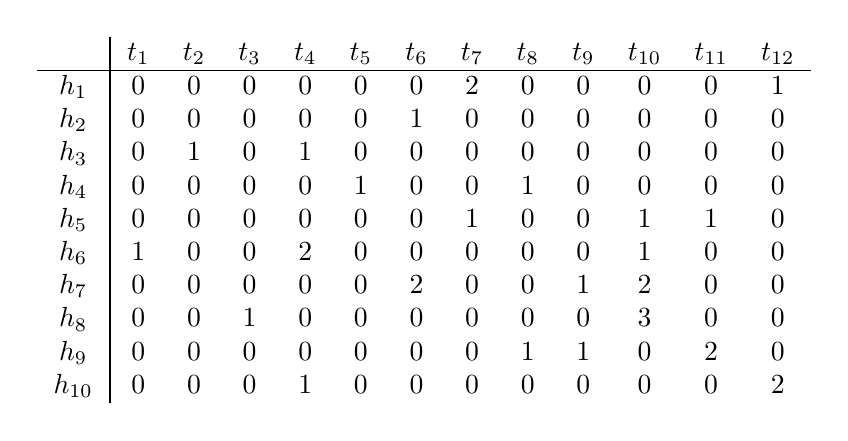
\begin{tikzpicture}[
    node distance=1cm,
    test/.style={circle, draw, thick, minimum size=0.6cm},
    decision/.style={circle, draw, thick, minimum size=0.55cm},
    leaf/.style={circle, draw, thick, fill=green!20, minimum size=0.5cm},
    arrow/.style={->, thick}
]

% Table of hypotheses vs tests (10 hypotheses, 12 tests, unbalanced outcomes)
\node[] at (0,0) {
\begin{tabular}{c|cccccccccccc}
 & $t_1$ & $t_2$ & $t_3$ & $t_4$ & $t_5$ & $t_6$ & $t_7$ & $t_8$ & $t_9$ & $t_{10}$ & $t_{11}$ & $t_{12}$ \\
\hline
$h_1$ & 0 & 0 & 0 & 0 & 0 & 0 & 2 & 0 & 0 & 0 & 0 & 1 \\
$h_2$ & 0 & 0 & 0 & 0 & 0 & 1 & 0 & 0 & 0 & 0 & 0 & 0 \\
$h_3$ & 0 & 1 & 0 & 1 & 0 & 0 & 0 & 0 & 0 & 0 & 0 & 0 \\
$h_4$ & 0 & 0 & 0 & 0 & 1 & 0 & 0 & 1 & 0 & 0 & 0 & 0 \\
$h_5$ & 0 & 0 & 0 & 0 & 0 & 0 & 1 & 0 & 0 & 1 & 1 & 0 \\
$h_6$ & 1 & 0 & 0 & 2 & 0 & 0 & 0 & 0 & 0 & 1 & 0 & 0 \\
$h_7$ & 0 & 0 & 0 & 0 & 0 & 2 & 0 & 0 & 1 & 2 & 0 & 0 \\
$h_8$ & 0 & 0 & 1 & 0 & 0 & 0 & 0 & 0 & 0 & 3 & 0 & 0 \\
$h_9$ & 0 & 0 & 0 & 0 & 0 & 0 & 0 & 1 & 1 & 0 & 2 & 0 \\
$h_{10}$ & 0 & 0 & 0 & 1 & 0 & 0 & 0 & 0 & 0 & 0 & 0 & 2 \\
\end{tabular}
};

\end{tikzpicture}
}
\normalsize
\caption*{(a) Hypotheses and tests table}
\end{minipage}

\begin{minipage}[t]{0.43\textwidth}
\centering
\scalebox{0.78}{
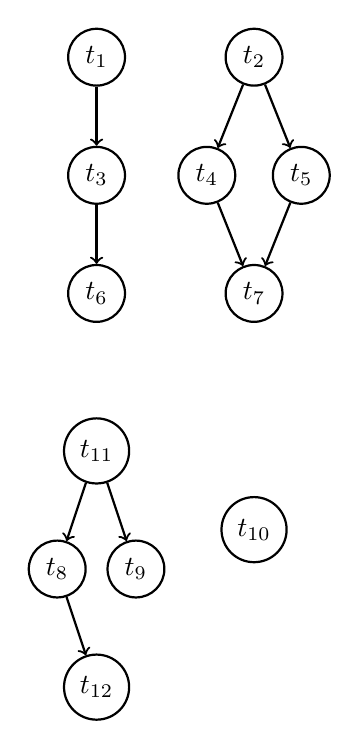
\begin{tikzpicture}[
    node distance=1cm,
    test/.style={circle, draw, thick, minimum size=0.6cm},
    arrow/.style={->, thick}
]

% DAG with 4 components (2 components on top, 2 below)
% Component 1 (top left)
\node[test] (t1) at (0.5,0) {$t_1$};
\node[test] (t3) at (0.5,-1.5) {$t_3$};
\node[test] (t6) at (0.5,-3) {$t_6$};
\draw[arrow] (t1) -- (t3);
\draw[arrow] (t3) -- (t6);

% Component 2 (top right)
\node[test] (t2) at (2.5,0) {$t_2$};
\node[test] (t4) at (1.9,-1.5) {$t_4$};
\node[test] (t5) at (3.1,-1.5) {$t_5$};
\node[test] (t7) at (2.5,-3) {$t_7$};
\draw[arrow] (t2) -- (t4);
\draw[arrow] (t2) -- (t5);
\draw[arrow] (t4) -- (t7);
\draw[arrow] (t5) -- (t7);

% Component 3 (bottom left)
\node[test] (t11) at (0.5,-5) {$t_{11}$};
\node[test] (t8) at (0,-6.5) {$t_8$};
\node[test] (t9) at (1,-6.5) {$t_9$};
\node[test] (t12) at (0.5,-8) {$t_{12}$};
\draw[arrow] (t11) -- (t8);
\draw[arrow] (t11) -- (t9);
\draw[arrow] (t8) -- (t12);

% Component 4 (isolated node, bottom right)
\node[test] (t10) at (2.5,-6) {$t_{10}$};

\end{tikzpicture}
}
\normalsize
\caption*{(b) Precedence}
\end{minipage}
\hfill
\begin{minipage}[t]{0.55\textwidth}
\centering
\scalebox{0.78}{
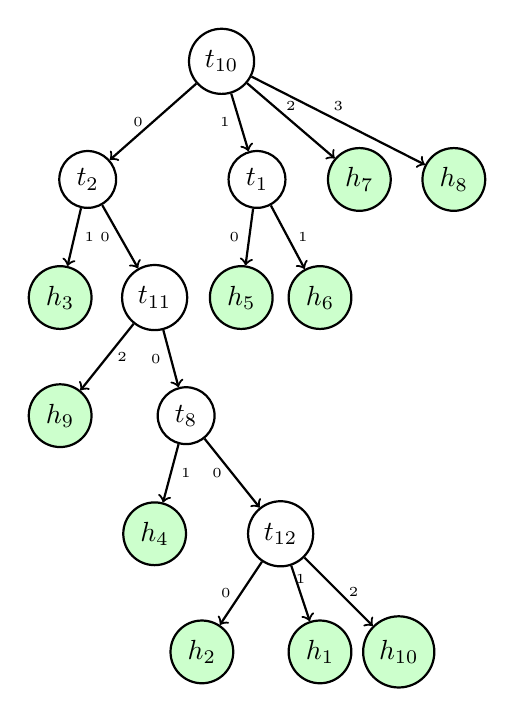
\begin{tikzpicture}[
    node distance=1cm,
    decision/.style={circle, draw, thick, minimum size=0.55cm},
    leaf/.style={circle, draw, thick, fill=green!20, minimum size=0.5cm},
    arrow/.style={->, thick}
]

% Decision tree built from table analysis
% Root: t10 (separates: h5→1, h6→1, h7→2, h8→3, rest→0)
\node[decision] (root) at (4.25,0) {$t_{10}$};

% t10=0: {h1,h2,h3,h4,h9,h10}
\node[decision] (n1) at (2.55,-1.5) {$t_2$};
% t10=1: {h5,h6}
\node[decision] (n2) at (4.7,-1.5) {$t_1$};
% t10=2: {h7}
\node[leaf] (h7) at (6,-1.5) {$h_7$};
% t10=3: {h8}
\node[leaf] (h8) at (7.2,-1.5) {$h_8$};

% t10=0, t2=0: {h1,h2,h4,h9,h10}
\node[decision] (n3) at (3.4,-3) {$t_{11}$};
% t10=0, t2=1: {h3}
\node[leaf] (h3) at (2.2,-3) {$h_3$};

% t10=1, t1=0: {h5}
\node[leaf] (h5) at (4.5,-3) {$h_5$};
% t10=1, t1=1: {h6}
\node[leaf] (h6) at (5.5,-3) {$h_6$};

% t10=0, t2=0, t11=0: {h1,h2,h4,h10}
\node[decision] (n4) at (3.8,-4.5) {$t_8$};
% t10=0, t2=0, t11=1: {h5} - but h5 already separated
% t10=0, t2=0, t11=2: {h9}
\node[leaf] (h9) at (2.2,-4.5) {$h_9$};

% t10=0, t2=0, t11=0, t8=0: {h1,h2,h10}
\node[decision] (n5) at (5,-6) {$t_{12}$};
% t10=0, t2=0, t11=0, t8=1: {h4}
\node[leaf] (h4) at (3.4,-6) {$h_4$};

% t10=0, t2=0, t11=0, t8=0, t12=0: {h2}
\node[leaf] (h2) at (4,-7.5) {$h_2$};
% t10=0, t2=0, t11=0, t8=0, t12=1: {h1}
\node[leaf] (h1) at (5.5,-7.5) {$h_1$};
% t10=0, t2=0, t11=0, t8=0, t12=2: {h10}
\node[leaf] (h10) at (6.5,-7.5) {$h_{10}$};

% Edges
\draw[arrow] (root) -- (n1) node[midway, left, font=\tiny] {0};
\draw[arrow] (root) -- (n2) node[midway, left, font=\tiny] {1};
\draw[arrow] (root) -- (h7) node[midway, above, font=\tiny] {2};
\draw[arrow] (root) -- (h8) node[midway, above, font=\tiny] {3};

\draw[arrow] (n1) -- (n3) node[midway, left, font=\tiny] {0};
\draw[arrow] (n1) -- (h3) node[midway, right, font=\tiny] {1};

\draw[arrow] (n2) -- (h5) node[midway, left, font=\tiny] {0};
\draw[arrow] (n2) -- (h6) node[midway, right, font=\tiny] {1};

\draw[arrow] (n3) -- (n4) node[midway, left, font=\tiny] {0};
\draw[arrow] (n3) -- (h9) node[midway, right, font=\tiny] {2};

\draw[arrow] (n4) -- (n5) node[midway, left, font=\tiny] {0};
\draw[arrow] (n4) -- (h4) node[midway, right, font=\tiny] {1};

\draw[arrow] (n5) -- (h2) node[midway, left, font=\tiny] {0};
\draw[arrow] (n5) -- (h1) node[midway, above, font=\tiny] {1};
\draw[arrow] (n5) -- (h10) node[midway, right, font=\tiny] {2};

\end{tikzpicture}
}
\normalsize
\caption*{(c) Valid decision tree}
\end{minipage}

% \caption{Example of a $\ProblemPCAL$ instance with 10 hypotheses and 12 tests. (a) Hypotheses-tests table. (b) Precedence DAG with four components. (c) A valid decision tree solution respecting precedence constraints.}\label{fig:pcal_example}
% \end{figure}
%
% \DD{na razie zakomentowałem rysunek dot zbiorów}
% \begin{figure}[h]
% \centering
% \centering

\begin{minipage}[t]{0.6\textwidth}
\centering
\scalebox{0.57}{
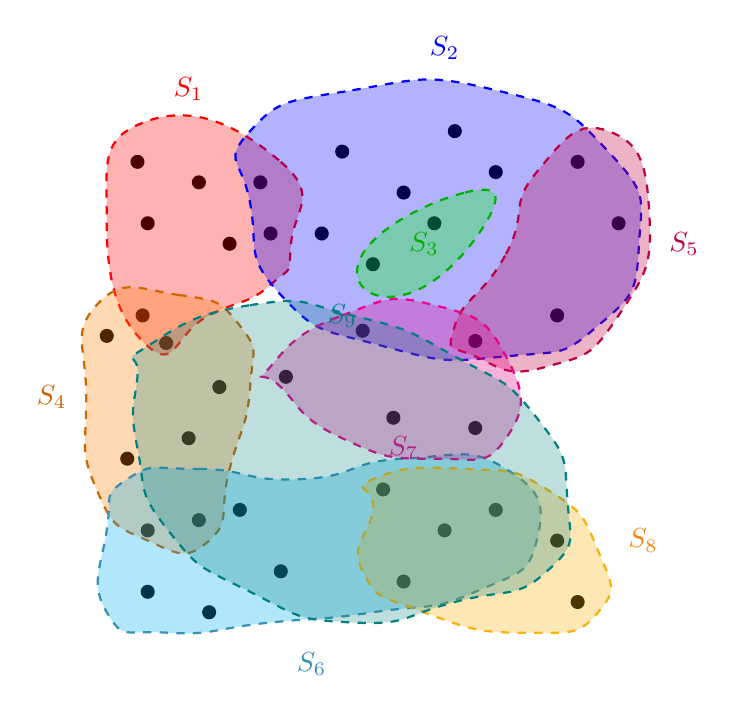
\begin{tikzpicture}[
    scale=1.3,
    node distance=1cm,
    element/.style={circle, draw, thick, fill=black, minimum size=0.15cm, inner sep=0pt},
    arrow/.style={->, thick}
]

% Universe elements - scattered randomly across the plane (35 elements with varied distribution)
\node[element] at (0.4, 3.9) {};
\node[element] at (0.9, 4.3) {};
\node[element] at (1.2, 3.7) {};
\node[element] at (0.35, 3) {};
\node[element] at (1.5, 4.3) {};
\node[element] at (0.3, 4.5) {};
\node[element] at (1.6, 3.8) {};  % SHARED by S1 and S2
\node[element] at (0.58, 2.73) {};  % SHARED by S1 and S4

\node[element] at (2.3, 4.6) {};
\node[element] at (2.9, 4.2) {};
\node[element] at (2.1, 3.8) {};
\node[element] at (3.4, 4.8) {};
\node[element] at (3.8, 4.4) {};
\node[element] at (2.6, 3.5) {};
\node[element] at (3.2, 3.9) {};

\node[element] at (4.6, 4.5) {};
\node[element] at (5, 3.9) {};
\node[element] at (4.4, 3) {};

\node[element] at (0, 2.8) {};
\node[element] at (1.1, 2.3) {};
\node[element] at (0.8, 1.8) {};
\node[element] at (0.2, 1.6) {};

\node[element] at (2.5, 2.85) {};
\node[element] at (3.6, 1.9) {};
\node[element] at (2.8, 2) {};
\node[element] at (3.6, 2.75) {};
\node[element] at (1.75, 2.4) {};

\node[element] at (0.9, 1.0) {};  % SHARED by S4 and S6
\node[element] at (0.4, 0.9) {};
\node[element] at (1.3, 1.1) {};
\node[element] at (0.4, 0.3) {};
\node[element] at (1.7, 0.5) {};
\node[element] at (1.0, 0.1) {};

\node[element] at (2.7, 1.3) {};
\node[element] at (3.3, 0.9) {};
\node[element] at (2.9, 0.4) {};
\node[element] at (3.8, 1.1) {};
\node[element] at (4.4, 0.8) {};
\node[element] at (4.6, 0.2) {};

% Set S1 (red) - includes (0.4,3.9) (0.9,4.3) (1.2,3.7) (0.6,3.2) (1.5,4.1) (0.3,4.5) + SHARED (1.6,4.0) (0.9,2.9)
\draw[thick, dashed, red, fill=red, fill opacity=0.3] 
    plot[smooth cycle, tension=1.0] coordinates {(0.4,4.9) (1.7,4.5) (1.8,3.7) (1.6,3.3) (1.0, 3) (0.4,2.7) (0.0,3.9)};
\node[above] at (0.8,5.0) {\textcolor{red}{$S_1$}};

% Set S2 (blue) - includes (2.3,4.6) (2.9,4.2) (2.1,3.8) (3.4,4.8) (3.8,4.4) (2.6,3.5) (3.2,3.9) (4.3,4.5) (4.7,3.9) (4.1,3.4) + SHARED (1.6,4.0)
\draw[thick, dashed, blue, fill=blue, fill opacity=0.3]
    plot[smooth cycle, tension=1.0] coordinates {(1.4,4.8) (2.4,5.2) (3.8,5.2) (4.9,4.6) (5.2,3.7) (4.8,2.9) (3.9,2.6) (2.7,2.7) (1.7,3.2) (1.4,4.1)};
\node[above] at (3.3,5.4) {\textcolor{blue}{$S_2$}};

% Set S3 (green) - small subset inside S2: (2.6,3.5) (3.2,3.9)
\draw[thick, dashed, green!70!black, fill=green, fill opacity=0.3]
    plot[smooth cycle, tension=1.0] coordinates {(2.5,3.6) (3.5,4.2) (3.7,3.9) (2.9,3.2)};
\node at (3.1,3.7) {\textcolor{green!70!black}{$S_3$}};

% Set S4 (orange) - includes (0.5,2.5) (1.1,2.8) (0.8,2.0) (0.2,1.6) + SHARED (0.9,1.0) (0.9,2.9)
\draw[thick, dashed, orange!80!black, fill=orange, fill opacity=0.3]
    plot[smooth cycle, tension=1.0] coordinates {(-0.1,3.1) (0.7,3.2) (1.3,2.9) (1.4,2.3) (1.2,1.5) (1.0,0.8) (0.4,0.8) (-0.1,1.3) (-0.2,2.2)};
\node[left] at (-0.3,2.2) {\textcolor{orange!80!black}{$S_4$}};

% Set S5 (purple) - right side elongated: (3.6,2.6) overlaps with S2 for (4.3,4.5) (4.7,3.9) (4.1,3.4)
\draw[thick, dashed, purple, fill=purple, fill opacity=0.3]
    plot[smooth cycle, tension=1.0] coordinates {(3.4,2.9) (3.9,3.6) (4.2,4.4) (4.9,4.8) (5.3,4.0) (5.0,3.0) (4.3,2.5) (3.6,2.6)};
\node[right] at (5.4,3.7) {\textcolor{purple}{$S_5$}};

% Set S6 (cyan) - includes (0.9,1.0) (0.7,0.8) (1.3,1.1) (0.4,0.3) (1.7,0.5) (1.0,0.1) (2.7,1.3) (3.3,0.9) (2.9,0.4) (3.8,1.1)
\draw[thick, dashed, cyan!70!black, fill=cyan, fill opacity=0.3]
    plot[smooth cycle, tension=1.0] coordinates {(0.2,1.4) (0.9,1.5) (1.9,1.4) (2.9,1.6) (3.9,1.5) (4.2,0.8) (3.6,0.3) (2.6,0.1) (1.6,0.0) (0.6,-0.1) (0.0,0.1) (0.0,0.9)};
\node[below] at (2.0,-0.2) {\textcolor{cyan!70!black}{$S_6$}};

% Set S7 (magenta) - includes (2.5,2.9) (3.1,2.4) (2.8,1.9) (1.9,2.2)
\draw[thick, dashed, magenta, fill=magenta, fill opacity=0.3]
    plot[smooth cycle, tension=1.0] coordinates {(1.6,2.5) (2.3,3.0) (3.2,3.1) (3.9,2.6) (3.9,1.8) (3.2,1.6) (2.3,1.8) (1.7,2.3)};
\node[above] at (2.9,1.5) {\textcolor{magenta}{$S_7$}};

% Set S8 (yellow!70!red) - includes (3.8,1.1) (4.4,0.6) (3.3,0.9) (2.9,0.4)
\draw[thick, dashed, yellow!70!red, fill=yellow!70!red, fill opacity=0.3]
    plot[smooth cycle, tension=1.0] coordinates {(2.6,1.4) (3.5,1.5) (4.3,1.3) (4.8,0.7) (4.8,0.1) (4.1,-0.1) (3.1,0.1) (2.5,0.5) (2.6,1.1)};
\node[right] at (5.0,0.8) {\textcolor{yellow!50!red}{$S_8$}};

% Set S9 (teal) - large blob filling gaps: overlaps with others to ensure complete coverage
\draw[thick, dashed, teal, fill=teal, fill opacity=0.25]
    plot[smooth cycle, tension=1.0] coordinates {(0.4,2.7) (1.4,3.1) (2.4,3.0) (3.4,2.6) (4.2,2.0) (4.5,1.2) (4.3,0.5) (3.4,0.2) (2.4,0.0) (1.4,0.3) (0.6,0.9) (0.3,1.7) (0.3,2.4)};
\node[below] at (2.3,3.2) {\textcolor{teal}{$S_9$}};

\end{tikzpicture}
}
\normalsize
\caption*{(a) Universe and sets}
\end{minipage}
\hfill
\begin{minipage}[t]{0.35\textwidth}
\centering
\scalebox{0.57}{
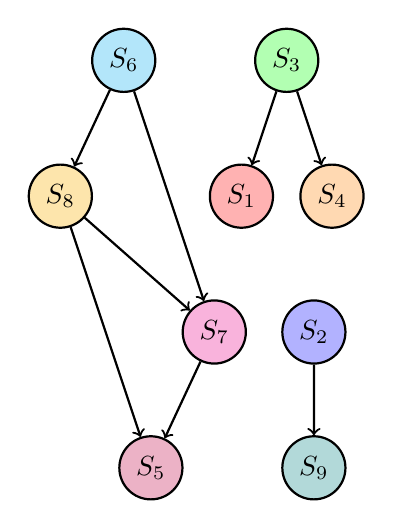
\begin{tikzpicture}[
    scale=1.15,
    node distance=1cm,
    set/.style={circle, draw, thick, minimum size=0.65cm},
    arrow/.style={->, thick}
]

% Precedence DAG with specified precedence constraints

% Component with S6 (left, wider)
\node[set, fill=cyan!30] (s6) at (0,0) {$S_6$};
\node[set, fill=yellow!70!red!30] (s8) at (-0.7,-1.5) {$S_8$};
\node[set, fill=magenta!30] (s7) at (1,-3) {$S_7$};
\node[set, fill=purple!30] (s5) at (0.3,-4.5) {$S_5$};

% Component with S3 (right top)
\node[set, fill=green!30] (s3) at (1.8,0) {$S_3$};
\node[set, fill=red!30] (s1) at (1.3,-1.5) {$S_1$};
\node[set, fill=orange!30] (s4) at (2.3,-1.5) {$S_4$};

% Component with S2 (right bottom)
\node[set, fill=blue!30] (s2) at (2.1,-3) {$S_2$};
\node[set, fill=teal!30] (s9) at (2.1,-4.5) {$S_9$};

% Precedence constraints (all arrows go down)
\draw[arrow] (s3) -- (s1);
\draw[arrow] (s3) -- (s4);
\draw[arrow] (s6) -- (s7);
\draw[arrow] (s6) -- (s8);
\draw[arrow] (s8) -- (s7);
\draw[arrow] (s8) -- (s5);
\draw[arrow] (s7) -- (s5);
\draw[arrow] (s2) -- (s9);

\end{tikzpicture}
}
\normalsize
\caption*{(b) Precedence}
\end{minipage}

\vspace{0.5cm}

\begin{minipage}[t]{\textwidth}
\centering
\scalebox{0.765}{
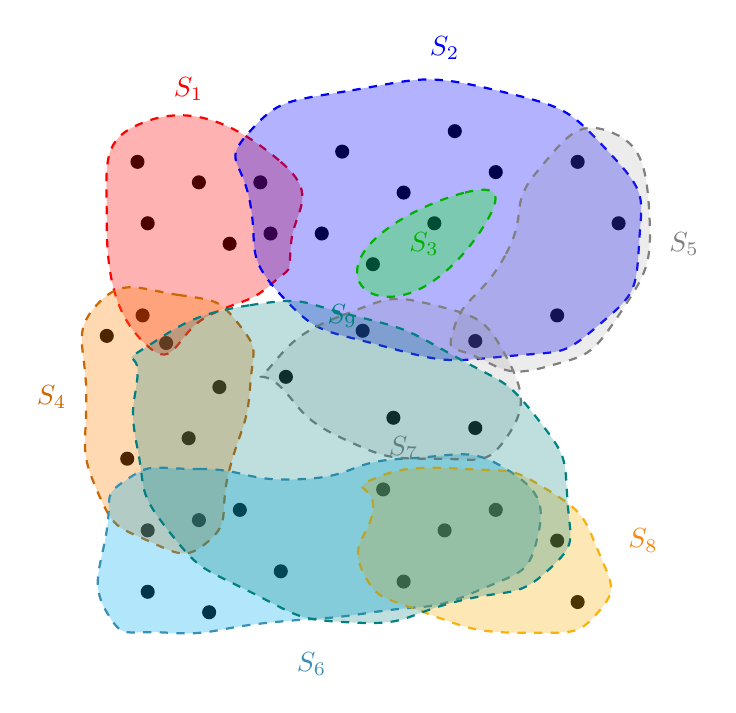
\begin{tikzpicture}[
    scale=1.3,
    node distance=1cm,
    element/.style={circle, draw, thick, fill=black, minimum size=0.15cm, inner sep=0pt},
    arrow/.style={->, thick}
]

% Universe elements - scattered randomly across the plane (35 elements with varied distribution)
\node[element] at (0.4, 3.9) {};
\node[element] at (0.9, 4.3) {};
\node[element] at (1.2, 3.7) {};
\node[element] at (0.35, 3) {};
\node[element] at (1.5, 4.3) {};
\node[element] at (0.3, 4.5) {};
\node[element] at (1.6, 3.8) {};  % SHARED by S1 and S2
\node[element] at (0.58, 2.73) {};  % SHARED by S1 and S4

\node[element] at (2.3, 4.6) {};
\node[element] at (2.9, 4.2) {};
\node[element] at (2.1, 3.8) {};
\node[element] at (3.4, 4.8) {};
\node[element] at (3.8, 4.4) {};
\node[element] at (2.6, 3.5) {};
\node[element] at (3.2, 3.9) {};

\node[element] at (4.6, 4.5) {};
\node[element] at (5, 3.9) {};
\node[element] at (4.4, 3) {};

\node[element] at (0, 2.8) {};
\node[element] at (1.1, 2.3) {};
\node[element] at (0.8, 1.8) {};
\node[element] at (0.2, 1.6) {};

\node[element] at (2.5, 2.85) {};
\node[element] at (3.6, 1.9) {};
\node[element] at (2.8, 2) {};
\node[element] at (3.6, 2.75) {};
\node[element] at (1.75, 2.4) {};

\node[element] at (0.9, 1.0) {};  % SHARED by S4 and S6
\node[element] at (0.4, 0.9) {};
\node[element] at (1.3, 1.1) {};
\node[element] at (0.4, 0.3) {};
\node[element] at (1.7, 0.5) {};
\node[element] at (1.0, 0.1) {};

\node[element] at (2.7, 1.3) {};
\node[element] at (3.3, 0.9) {};
\node[element] at (2.9, 0.4) {};
\node[element] at (3.8, 1.1) {};
\node[element] at (4.4, 0.8) {};
\node[element] at (4.6, 0.2) {};

% Set S1 (red) - SELECTED
\draw[thick, dashed, red, fill=red, fill opacity=0.3] 
    plot[smooth cycle, tension=1.0] coordinates {(0.4,4.9) (1.7,4.5) (1.8,3.7) (1.6,3.3) (1.0, 3) (0.4,2.7) (0.0,3.9)};
\node[above] at (0.8,5.0) {\textcolor{red}{\textbf{$S_1$}}};

% Set S2 (blue) - SELECTED
\draw[thick, dashed, blue, fill=blue, fill opacity=0.3]
    plot[smooth cycle, tension=1.0] coordinates {(1.4,4.8) (2.4,5.2) (3.8,5.2) (4.9,4.6) (5.2,3.7) (4.8,2.9) (3.9,2.6) (2.7,2.7) (1.7,3.2) (1.4,4.1)};
\node[above] at (3.3,5.4) {\textcolor{blue}{\textbf{$S_2$}}};

% Set S3 (green) - SELECTED
\draw[thick, dashed, green!70!black, fill=green, fill opacity=0.3]
    plot[smooth cycle, tension=1.0] coordinates {(2.5,3.6) (3.5,4.2) (3.7,3.9) (2.9,3.2)};
\node at (3.1,3.7) {\textcolor{green!70!black}{\textbf{$S_3$}}};

% Set S4 (orange) - SELECTED
\draw[thick, dashed, orange!80!black, fill=orange, fill opacity=0.3]
    plot[smooth cycle, tension=1.0] coordinates {(-0.1,3.1) (0.7,3.2) (1.3,2.9) (1.4,2.3) (1.2,1.5) (1.0,0.8) (0.4,0.8) (-0.1,1.3) (-0.2,2.2)};
\node[left] at (-0.3,2.2) {\textcolor{orange!80!black}{\textbf{$S_4$}}};

% Set S5 (purple) - NOT SELECTED (grayed out)
\draw[thick, dashed, gray, fill=gray, fill opacity=0.15]
    plot[smooth cycle, tension=1.0] coordinates {(3.4,2.9) (3.9,3.6) (4.2,4.4) (4.9,4.8) (5.3,4.0) (5.0,3.0) (4.3,2.5) (3.6,2.6)};
\node[right] at (5.4,3.7) {\textcolor{gray}{$S_5$}};

% Set S6 (cyan) - SELECTED
\draw[thick, dashed, cyan!70!black, fill=cyan, fill opacity=0.3]
    plot[smooth cycle, tension=1.0] coordinates {(0.2,1.4) (0.9,1.5) (1.9,1.4) (2.9,1.6) (3.9,1.5) (4.2,0.8) (3.6,0.3) (2.6,0.1) (1.6,0.0) (0.6,-0.1) (0.0,0.1) (0.0,0.9)};
\node[below] at (2.0,-0.2) {\textcolor{cyan!70!black}{\textbf{$S_6$}}};

% Set S7 (magenta) - NOT SELECTED (grayed out)
\draw[thick, dashed, gray, fill=gray, fill opacity=0.15]
    plot[smooth cycle, tension=1.0] coordinates {(1.6,2.5) (2.3,3.0) (3.2,3.1) (3.9,2.6) (3.9,1.8) (3.2,1.6) (2.3,1.8) (1.7,2.3)};
\node[above] at (2.9,1.5) {\textcolor{gray}{$S_7$}};

% Set S8 (yellow!70!red) - SELECTED
\draw[thick, dashed, yellow!70!red, fill=yellow!70!red, fill opacity=0.3]
    plot[smooth cycle, tension=1.0] coordinates {(2.6,1.4) (3.5,1.5) (4.3,1.3) (4.8,0.7) (4.8,0.1) (4.1,-0.1) (3.1,0.1) (2.5,0.5) (2.6,1.1)};
\node[right] at (5.0,0.8) {\textcolor{yellow!50!red}{\textbf{$S_8$}}};

% Set S9 (teal) - SELECTED
\draw[thick, dashed, teal, fill=teal, fill opacity=0.25]
    plot[smooth cycle, tension=1.0] coordinates {(0.4,2.7) (1.4,3.1) (2.4,3.0) (3.4,2.6) (4.2,2.0) (4.5,1.2) (4.3,0.5) (3.4,0.2) (2.4,0.0) (1.4,0.3) (0.6,0.9) (0.3,1.7) (0.3,2.4)};
\node[below] at (2.3,3.2) {\textcolor{teal}{\textbf{$S_9$}}};

\end{tikzpicture}
}
\normalsize
\caption*{(c) Solution: $\{S_1, S_2, S_6, S_8, S_9\}$ (in color)}
\end{minipage}


% \caption{Example of a PCCP instance with 39 elements and 9 covering sets. (a) Universe with covering sets. (b) Precedence DAG with three components. (c) Solution using 7 selected sets (colored).}\label{fig:pccp_example}
% \end{figure}

% \begin{figure}[h]
% \centering
% \centering

\begin{minipage}[t]{0.6\textwidth}
\centering
\scalebox{0.57}{
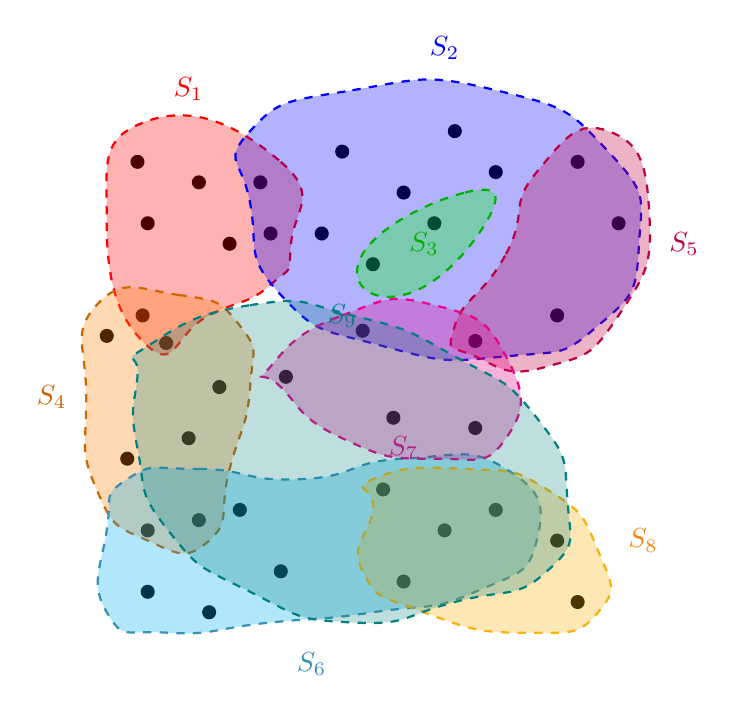
\begin{tikzpicture}[
    scale=1.3,
    node distance=1cm,
    element/.style={circle, draw, thick, fill=black, minimum size=0.15cm, inner sep=0pt},
    arrow/.style={->, thick}
]

% Universe elements - scattered randomly across the plane (35 elements with varied distribution)
\node[element] at (0.4, 3.9) {};
\node[element] at (0.9, 4.3) {};
\node[element] at (1.2, 3.7) {};
\node[element] at (0.35, 3) {};
\node[element] at (1.5, 4.3) {};
\node[element] at (0.3, 4.5) {};
\node[element] at (1.6, 3.8) {};  % SHARED by S1 and S2
\node[element] at (0.58, 2.73) {};  % SHARED by S1 and S4

\node[element] at (2.3, 4.6) {};
\node[element] at (2.9, 4.2) {};
\node[element] at (2.1, 3.8) {};
\node[element] at (3.4, 4.8) {};
\node[element] at (3.8, 4.4) {};
\node[element] at (2.6, 3.5) {};
\node[element] at (3.2, 3.9) {};

\node[element] at (4.6, 4.5) {};
\node[element] at (5, 3.9) {};
\node[element] at (4.4, 3) {};

\node[element] at (0, 2.8) {};
\node[element] at (1.1, 2.3) {};
\node[element] at (0.8, 1.8) {};
\node[element] at (0.2, 1.6) {};

\node[element] at (2.5, 2.85) {};
\node[element] at (3.6, 1.9) {};
\node[element] at (2.8, 2) {};
\node[element] at (3.6, 2.75) {};
\node[element] at (1.75, 2.4) {};

\node[element] at (0.9, 1.0) {};  % SHARED by S4 and S6
\node[element] at (0.4, 0.9) {};
\node[element] at (1.3, 1.1) {};
\node[element] at (0.4, 0.3) {};
\node[element] at (1.7, 0.5) {};
\node[element] at (1.0, 0.1) {};

\node[element] at (2.7, 1.3) {};
\node[element] at (3.3, 0.9) {};
\node[element] at (2.9, 0.4) {};
\node[element] at (3.8, 1.1) {};
\node[element] at (4.4, 0.8) {};
\node[element] at (4.6, 0.2) {};

% Set S1 (red) - includes (0.4,3.9) (0.9,4.3) (1.2,3.7) (0.6,3.2) (1.5,4.1) (0.3,4.5) + SHARED (1.6,4.0) (0.9,2.9)
\draw[thick, dashed, red, fill=red, fill opacity=0.3] 
    plot[smooth cycle, tension=1.0] coordinates {(0.4,4.9) (1.7,4.5) (1.8,3.7) (1.6,3.3) (1.0, 3) (0.4,2.7) (0.0,3.9)};
\node[above] at (0.8,5.0) {\textcolor{red}{$S_1$}};

% Set S2 (blue) - includes (2.3,4.6) (2.9,4.2) (2.1,3.8) (3.4,4.8) (3.8,4.4) (2.6,3.5) (3.2,3.9) (4.3,4.5) (4.7,3.9) (4.1,3.4) + SHARED (1.6,4.0)
\draw[thick, dashed, blue, fill=blue, fill opacity=0.3]
    plot[smooth cycle, tension=1.0] coordinates {(1.4,4.8) (2.4,5.2) (3.8,5.2) (4.9,4.6) (5.2,3.7) (4.8,2.9) (3.9,2.6) (2.7,2.7) (1.7,3.2) (1.4,4.1)};
\node[above] at (3.3,5.4) {\textcolor{blue}{$S_2$}};

% Set S3 (green) - small subset inside S2: (2.6,3.5) (3.2,3.9)
\draw[thick, dashed, green!70!black, fill=green, fill opacity=0.3]
    plot[smooth cycle, tension=1.0] coordinates {(2.5,3.6) (3.5,4.2) (3.7,3.9) (2.9,3.2)};
\node at (3.1,3.7) {\textcolor{green!70!black}{$S_3$}};

% Set S4 (orange) - includes (0.5,2.5) (1.1,2.8) (0.8,2.0) (0.2,1.6) + SHARED (0.9,1.0) (0.9,2.9)
\draw[thick, dashed, orange!80!black, fill=orange, fill opacity=0.3]
    plot[smooth cycle, tension=1.0] coordinates {(-0.1,3.1) (0.7,3.2) (1.3,2.9) (1.4,2.3) (1.2,1.5) (1.0,0.8) (0.4,0.8) (-0.1,1.3) (-0.2,2.2)};
\node[left] at (-0.3,2.2) {\textcolor{orange!80!black}{$S_4$}};

% Set S5 (purple) - right side elongated: (3.6,2.6) overlaps with S2 for (4.3,4.5) (4.7,3.9) (4.1,3.4)
\draw[thick, dashed, purple, fill=purple, fill opacity=0.3]
    plot[smooth cycle, tension=1.0] coordinates {(3.4,2.9) (3.9,3.6) (4.2,4.4) (4.9,4.8) (5.3,4.0) (5.0,3.0) (4.3,2.5) (3.6,2.6)};
\node[right] at (5.4,3.7) {\textcolor{purple}{$S_5$}};

% Set S6 (cyan) - includes (0.9,1.0) (0.7,0.8) (1.3,1.1) (0.4,0.3) (1.7,0.5) (1.0,0.1) (2.7,1.3) (3.3,0.9) (2.9,0.4) (3.8,1.1)
\draw[thick, dashed, cyan!70!black, fill=cyan, fill opacity=0.3]
    plot[smooth cycle, tension=1.0] coordinates {(0.2,1.4) (0.9,1.5) (1.9,1.4) (2.9,1.6) (3.9,1.5) (4.2,0.8) (3.6,0.3) (2.6,0.1) (1.6,0.0) (0.6,-0.1) (0.0,0.1) (0.0,0.9)};
\node[below] at (2.0,-0.2) {\textcolor{cyan!70!black}{$S_6$}};

% Set S7 (magenta) - includes (2.5,2.9) (3.1,2.4) (2.8,1.9) (1.9,2.2)
\draw[thick, dashed, magenta, fill=magenta, fill opacity=0.3]
    plot[smooth cycle, tension=1.0] coordinates {(1.6,2.5) (2.3,3.0) (3.2,3.1) (3.9,2.6) (3.9,1.8) (3.2,1.6) (2.3,1.8) (1.7,2.3)};
\node[above] at (2.9,1.5) {\textcolor{magenta}{$S_7$}};

% Set S8 (yellow!70!red) - includes (3.8,1.1) (4.4,0.6) (3.3,0.9) (2.9,0.4)
\draw[thick, dashed, yellow!70!red, fill=yellow!70!red, fill opacity=0.3]
    plot[smooth cycle, tension=1.0] coordinates {(2.6,1.4) (3.5,1.5) (4.3,1.3) (4.8,0.7) (4.8,0.1) (4.1,-0.1) (3.1,0.1) (2.5,0.5) (2.6,1.1)};
\node[right] at (5.0,0.8) {\textcolor{yellow!50!red}{$S_8$}};

% Set S9 (teal) - large blob filling gaps: overlaps with others to ensure complete coverage
\draw[thick, dashed, teal, fill=teal, fill opacity=0.25]
    plot[smooth cycle, tension=1.0] coordinates {(0.4,2.7) (1.4,3.1) (2.4,3.0) (3.4,2.6) (4.2,2.0) (4.5,1.2) (4.3,0.5) (3.4,0.2) (2.4,0.0) (1.4,0.3) (0.6,0.9) (0.3,1.7) (0.3,2.4)};
\node[below] at (2.3,3.2) {\textcolor{teal}{$S_9$}};

\end{tikzpicture}
}
\normalsize
\caption*{(a) Universe and sets}
\end{minipage}
\hfill
\begin{minipage}[t]{0.35\textwidth}
\centering
\scalebox{0.57}{
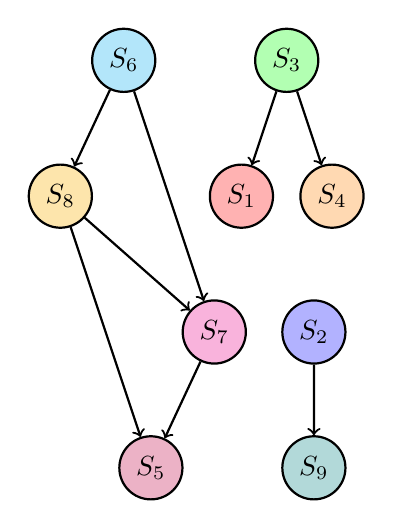
\begin{tikzpicture}[
    scale=1.15,
    node distance=1cm,
    set/.style={circle, draw, thick, minimum size=0.65cm},
    arrow/.style={->, thick}
]

% Precedence DAG with specified precedence constraints

% Component with S6 (left, wider)
\node[set, fill=cyan!30] (s6) at (0,0) {$S_6$};
\node[set, fill=yellow!70!red!30] (s8) at (-0.7,-1.5) {$S_8$};
\node[set, fill=magenta!30] (s7) at (1,-3) {$S_7$};
\node[set, fill=purple!30] (s5) at (0.3,-4.5) {$S_5$};

% Component with S3 (right top)
\node[set, fill=green!30] (s3) at (1.8,0) {$S_3$};
\node[set, fill=red!30] (s1) at (1.3,-1.5) {$S_1$};
\node[set, fill=orange!30] (s4) at (2.3,-1.5) {$S_4$};

% Component with S2 (right bottom)
\node[set, fill=blue!30] (s2) at (2.1,-3) {$S_2$};
\node[set, fill=teal!30] (s9) at (2.1,-4.5) {$S_9$};

% Precedence constraints (all arrows go down)
\draw[arrow] (s3) -- (s1);
\draw[arrow] (s3) -- (s4);
\draw[arrow] (s6) -- (s7);
\draw[arrow] (s6) -- (s8);
\draw[arrow] (s8) -- (s7);
\draw[arrow] (s8) -- (s5);
\draw[arrow] (s7) -- (s5);
\draw[arrow] (s2) -- (s9);

\end{tikzpicture}
}
\normalsize
\caption*{(b) Precedence}
\end{minipage}

\vspace{0.5cm}

\begin{minipage}[t]{\textwidth}
\centering
\scalebox{0.765}{
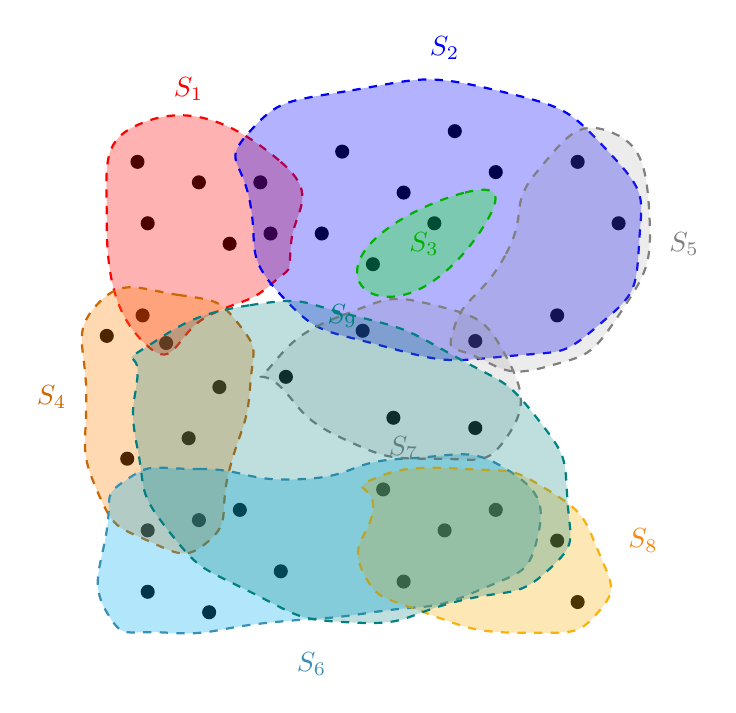
\begin{tikzpicture}[
    scale=1.3,
    node distance=1cm,
    element/.style={circle, draw, thick, fill=black, minimum size=0.15cm, inner sep=0pt},
    arrow/.style={->, thick}
]

% Universe elements - scattered randomly across the plane (35 elements with varied distribution)
\node[element] at (0.4, 3.9) {};
\node[element] at (0.9, 4.3) {};
\node[element] at (1.2, 3.7) {};
\node[element] at (0.35, 3) {};
\node[element] at (1.5, 4.3) {};
\node[element] at (0.3, 4.5) {};
\node[element] at (1.6, 3.8) {};  % SHARED by S1 and S2
\node[element] at (0.58, 2.73) {};  % SHARED by S1 and S4

\node[element] at (2.3, 4.6) {};
\node[element] at (2.9, 4.2) {};
\node[element] at (2.1, 3.8) {};
\node[element] at (3.4, 4.8) {};
\node[element] at (3.8, 4.4) {};
\node[element] at (2.6, 3.5) {};
\node[element] at (3.2, 3.9) {};

\node[element] at (4.6, 4.5) {};
\node[element] at (5, 3.9) {};
\node[element] at (4.4, 3) {};

\node[element] at (0, 2.8) {};
\node[element] at (1.1, 2.3) {};
\node[element] at (0.8, 1.8) {};
\node[element] at (0.2, 1.6) {};

\node[element] at (2.5, 2.85) {};
\node[element] at (3.6, 1.9) {};
\node[element] at (2.8, 2) {};
\node[element] at (3.6, 2.75) {};
\node[element] at (1.75, 2.4) {};

\node[element] at (0.9, 1.0) {};  % SHARED by S4 and S6
\node[element] at (0.4, 0.9) {};
\node[element] at (1.3, 1.1) {};
\node[element] at (0.4, 0.3) {};
\node[element] at (1.7, 0.5) {};
\node[element] at (1.0, 0.1) {};

\node[element] at (2.7, 1.3) {};
\node[element] at (3.3, 0.9) {};
\node[element] at (2.9, 0.4) {};
\node[element] at (3.8, 1.1) {};
\node[element] at (4.4, 0.8) {};
\node[element] at (4.6, 0.2) {};

% Set S1 (red) - SELECTED
\draw[thick, dashed, red, fill=red, fill opacity=0.3] 
    plot[smooth cycle, tension=1.0] coordinates {(0.4,4.9) (1.7,4.5) (1.8,3.7) (1.6,3.3) (1.0, 3) (0.4,2.7) (0.0,3.9)};
\node[above] at (0.8,5.0) {\textcolor{red}{\textbf{$S_1$}}};

% Set S2 (blue) - SELECTED
\draw[thick, dashed, blue, fill=blue, fill opacity=0.3]
    plot[smooth cycle, tension=1.0] coordinates {(1.4,4.8) (2.4,5.2) (3.8,5.2) (4.9,4.6) (5.2,3.7) (4.8,2.9) (3.9,2.6) (2.7,2.7) (1.7,3.2) (1.4,4.1)};
\node[above] at (3.3,5.4) {\textcolor{blue}{\textbf{$S_2$}}};

% Set S3 (green) - SELECTED
\draw[thick, dashed, green!70!black, fill=green, fill opacity=0.3]
    plot[smooth cycle, tension=1.0] coordinates {(2.5,3.6) (3.5,4.2) (3.7,3.9) (2.9,3.2)};
\node at (3.1,3.7) {\textcolor{green!70!black}{\textbf{$S_3$}}};

% Set S4 (orange) - SELECTED
\draw[thick, dashed, orange!80!black, fill=orange, fill opacity=0.3]
    plot[smooth cycle, tension=1.0] coordinates {(-0.1,3.1) (0.7,3.2) (1.3,2.9) (1.4,2.3) (1.2,1.5) (1.0,0.8) (0.4,0.8) (-0.1,1.3) (-0.2,2.2)};
\node[left] at (-0.3,2.2) {\textcolor{orange!80!black}{\textbf{$S_4$}}};

% Set S5 (purple) - NOT SELECTED (grayed out)
\draw[thick, dashed, gray, fill=gray, fill opacity=0.15]
    plot[smooth cycle, tension=1.0] coordinates {(3.4,2.9) (3.9,3.6) (4.2,4.4) (4.9,4.8) (5.3,4.0) (5.0,3.0) (4.3,2.5) (3.6,2.6)};
\node[right] at (5.4,3.7) {\textcolor{gray}{$S_5$}};

% Set S6 (cyan) - SELECTED
\draw[thick, dashed, cyan!70!black, fill=cyan, fill opacity=0.3]
    plot[smooth cycle, tension=1.0] coordinates {(0.2,1.4) (0.9,1.5) (1.9,1.4) (2.9,1.6) (3.9,1.5) (4.2,0.8) (3.6,0.3) (2.6,0.1) (1.6,0.0) (0.6,-0.1) (0.0,0.1) (0.0,0.9)};
\node[below] at (2.0,-0.2) {\textcolor{cyan!70!black}{\textbf{$S_6$}}};

% Set S7 (magenta) - NOT SELECTED (grayed out)
\draw[thick, dashed, gray, fill=gray, fill opacity=0.15]
    plot[smooth cycle, tension=1.0] coordinates {(1.6,2.5) (2.3,3.0) (3.2,3.1) (3.9,2.6) (3.9,1.8) (3.2,1.6) (2.3,1.8) (1.7,2.3)};
\node[above] at (2.9,1.5) {\textcolor{gray}{$S_7$}};

% Set S8 (yellow!70!red) - SELECTED
\draw[thick, dashed, yellow!70!red, fill=yellow!70!red, fill opacity=0.3]
    plot[smooth cycle, tension=1.0] coordinates {(2.6,1.4) (3.5,1.5) (4.3,1.3) (4.8,0.7) (4.8,0.1) (4.1,-0.1) (3.1,0.1) (2.5,0.5) (2.6,1.1)};
\node[right] at (5.0,0.8) {\textcolor{yellow!50!red}{\textbf{$S_8$}}};

% Set S9 (teal) - SELECTED
\draw[thick, dashed, teal, fill=teal, fill opacity=0.25]
    plot[smooth cycle, tension=1.0] coordinates {(0.4,2.7) (1.4,3.1) (2.4,3.0) (3.4,2.6) (4.2,2.0) (4.5,1.2) (4.3,0.5) (3.4,0.2) (2.4,0.0) (1.4,0.3) (0.6,0.9) (0.3,1.7) (0.3,2.4)};
\node[below] at (2.3,3.2) {\textcolor{teal}{\textbf{$S_9$}}};

\end{tikzpicture}
}
\normalsize
\caption*{(c) Solution: $\{S_1, S_2, S_6, S_8, S_9\}$ (in color)}
\end{minipage}


% \caption{Example of a PCCP instance with 39 elements and 9 covering sets. (a) Universe with covering sets. (b) Precedence DAG with three components. (c) Solution using 7 selected sets (colored).}\label{fig:pccp_example}
% \end{figure}

Table~\ref{tab:results} summarizes all results, also including best known from literature.
\begin{table}[htb]
\caption{Approximation guarantees for covering and decision tree problems under different precedence constraints. (* denotes new results, ** denotes previously unmentioned corollaries of known results).}
\label{tab:results}
\centering
{
\small
\begin{tabular}{lC{0.14\linewidth}C{0.14\linewidth}C{0.14\linewidth}C{0.14\linewidth}C{0.14\linewidth}}
\toprule
\textbf{precedence} & \textbf{$\ProblemPCSC$} & \textbf{$\ProblemBPCSC$} & \textbf{$\ProblemPCMSSC$} & \textbf{$\ProblemPCWCDT$} & \textbf{$\ProblemPCACDT$} \\
\midrule
none & $\cO(\log n)$ \cite{ThresholdLnNSetCover} & $\br{1, \frac{e}{e-1}}$ \cite{TheBudgetedMaximumCoverageProblem} & $4$ \cite{ApproximatingMinSumSetCover} & $\cO(\log n)$** & $\cO(\log n)$ \cite{ApproximatingDecisionTreesMultiwayBranches} \\
\midrule
inforest & $\br{1, \frac{e}{e-1}}$ (Thm.~\ref{thm:BPCSC-inforest}) & $\br{1, \frac{e}{e-1}}$ (Thm.~\ref{thm:BPCSC-inforest}) & $\cO(1)$* & $\cO(\log n)$* & $\cO(\log(m\!+\!n))$* \\
\midrule
outforest & $\br{\cO(\log n), 4}$ (Thm.~\ref{thm:BPCSC-outforest}) & $\br{\cO(\log n), 4}$ (Thm.~\ref{thm:BPCSC-outforest}) & $\br{\cO(\log n), 4}$* & $\cO(\log^2 n)$* & $\cO(\log^2(m\!+\!n))$* \\
\midrule
general & $\cO(\sqrt{m}f)$ (Thm.~\ref{thm:generalPCSC}) & $\br{\sqrt{m\cdot H_n}\!+\!1, 1}$ (Thm.~\ref{thm:BPCSC}) & $\cO(\sqrt{m})$ (Thm.~\ref{thm:generalPCMSSC}) & $\cO(\sqrt{m}\log n)$ (Thm.~\ref{thm:generalPCWCDT}) & $\cO(\sqrt{m}\log^{3/2}(m\!+\!n))$ (Thm.~\ref{thm:generalPCACDT}) \\
\bottomrule
\end{tabular}
}
\end{table}

\begin{figure}[h]
\centering
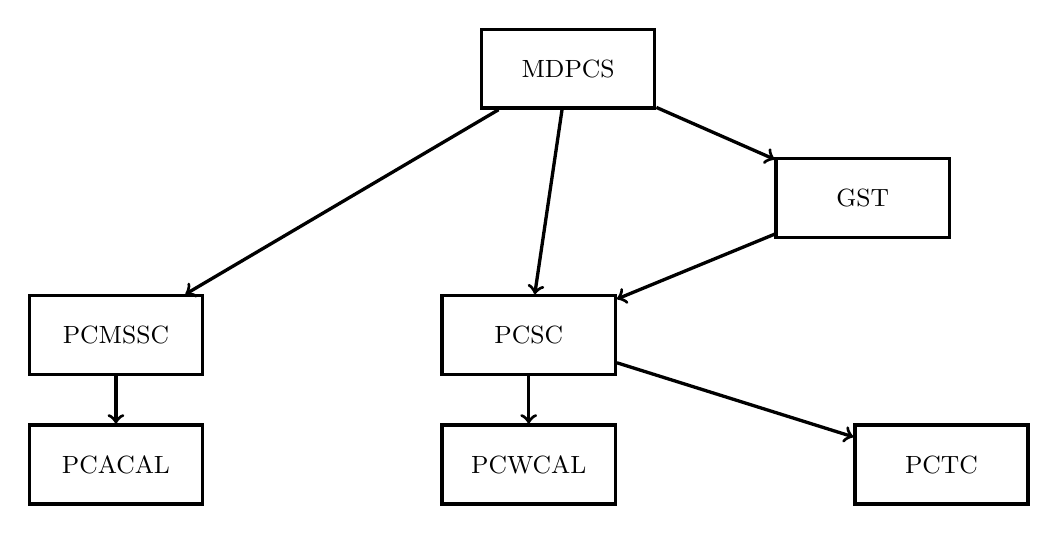
\begin{tikzpicture}[
    node distance=2.5cm and 3cm,
    problem/.style={rectangle, draw, very thick, minimum width=2.2cm, minimum height=1cm, align=center, font=\small},
    arrow/.style={->, very thick}
]

% Third row (define first for positioning)
\node[problem] (pcmssc) {PCMSSC};
\node[problem, right=3cm of pcmssc] (pcsc) {PCSC};

% Second row (above pcsc)
\node[problem, above right=0.7cm and 2cm of pcsc] (gst) {GST};

% Top row (above gst)
\node[problem, above left=0.6cm and 1.5cm of gst] (mdpcs) {MDPCS};

% Bottom row
\node[problem, below=0.6cm of pcmssc] (pcacal) {PCACAL};
\node[problem, below=0.6cm of pcsc] (pcwcal) {PCWCAL};
\node[problem, right=3cm of pcwcal] (pctc) {PCTC};

% Arrows
\draw[arrow] (mdpcs) -- (gst);
\draw[arrow] (mdpcs) -- (pcsc);
\draw[arrow] (mdpcs) -- (pcmssc);
\draw[arrow] (gst) -- (pcsc);
\draw[arrow] (pcsc) -- (pctc);
\draw[arrow] (pcsc) -- (pcwcal);
\draw[arrow] (pcmssc) -- (pcacal);

\end{tikzpicture}

\caption{Relationships between covering and decision tree problems, $\Pi_1 \to \Pi_2$ denotes that an approximation algorithm for problem $\Pi_1$ implies an approximation algorithm for problem $\Pi_2$.}\label{fig:reductions}
\end{figure}

\begin{figure}[h]
    \centering
    \begin{tikzpicture}[
    node distance=1.1cm and 2cm,
    problem/.style={rectangle, draw, very thick, minimum width=1.8cm, minimum height=0.8cm, align=center, font=\scriptsize},
    arrow/.style={->, very thick}
]

% Define positions based on the hand-drawn diagram
% Top level
\node[problem] (gst) at (-2, 0) {$\ProblemGST$};
\node[problem] (pds) at (2, 0) {$\ProblemPDS$};

% Middle level
\node[problem, below left=1.1cm and 0.5cm of pds] (fpcsc) {$\ProblemPCSC$};
\node[problem, below right=1.1cm and 0.5cm of pds] (fpcmssc) {$\ProblemPCMSSC$};

% Bottom level
\node[problem, below=1.1cm of fpcsc] (pcwcdt) {$\ProblemPCWCDT$};
\node[problem, below=1.1cm of fpcmssc] (pcacdt) {$\ProblemPCACDT$};

% Arrows with hyperlinks to sections
\draw[arrow] (gst) -- (fpcsc);
\draw[arrow] (pds) -- (fpcsc);
\draw[arrow] (pds) -- (fpcmssc);
\draw[arrow] (fpcsc) -- (pcwcdt);
\draw[arrow] (fpcsc) -- (pcacdt);
\draw[arrow] (fpcmssc) -- (pcacdt);

\end{tikzpicture}

    \caption{Inapproximability relations between problems, $\Pi_1 \to \Pi_2$ denotes that an inapproximability result for problem $\Pi_1$ implies an inapproximability result for problem $\Pi_2$.}
    \label{fig:hardness_diagram}
\end{figure}

\DD{tutaj bylby jakis wywod i intuicje jakie techniki sa nowe, generalnie trzebaby sie pochwalic pomyslami roznymi}

\subsection{Organization}
\section{Preliminaries}
\begin{definition}[Precedence constrained set cover (PCSC)]
Given a universe $\mathcal{U}$ of $n$ items, a collection $\mathcal{S}$ of $m$ subsets of $\mathcal{U}$, a DAG $\mathcal{F} = \brc{\mathcal{S}, \preceq}$ encoding precedence constraints, and a coverage requirement $K$, find a precedence-closed subfamily $\mathcal{C} \subseteq \mathcal{S}$ that covers at least $K$ items while minimizing $\spr{\mathcal{C}}$.
\end{definition}
\begin{definition}[Precedence constrained min-sum set cover (PCMSSC)]
Given a universe $\mathcal{U}$ of $n$ items, a collection $\mathcal{S}$ of $m$ subsets of $\mathcal{U}$, a DAG $\mathcal{F} = \brc{\mathcal{S}, \preceq}$ encoding precedence constraints, and a coverage requirement $K$, find a precedence-closed sequence of sets that covers at least $K$ items while minimizing the average time (position in sequence) at which items are covered.
\end{definition}
\begin{definition}[Precedence constrained test cover (PCTC)]
Given a set $\mathcal{H}$ of $n$ hypotheses, a set $\mathcal{T}$ of $m$ tests, and a DAG $\mathcal{F} = \brc{\mathcal{T}, \preceq}$ encoding precedence constraints, find a precedence-closed subfamily of tests that distinguishes all pairs of hypotheses.
\end{definition}
\begin{definition}[Precedence constrained worst case active learning (PCWCAL)]
Given a set $\mathcal{H}$ of $n$ hypotheses, a set $\mathcal{T}$ of $m$ tests, and a DAG $\mathcal{F} = \brc{\mathcal{T}, \preceq}$ encoding precedence constraints, construct a decision tree respecting precedence constraints that identifies any hypothesis from $\mathcal{H}$ while minimizing the worst-case depth of the tree.
\end{definition}
\begin{definition}[Precedence constrained average case active learning (PCACAL)]
Given a set $\mathcal{H}$ of $n$ hypotheses, a set $\mathcal{T}$ of $m$ tests, a DAG $\mathcal{F} = \brc{\mathcal{T}, \preceq}$ encoding precedence constraints, and a probability distribution over $\mathcal{H}$, construct a decision tree respecting precedence constraints that identifies any hypothesis from $\mathcal{H}$ while minimizing the expected depth (average case cost).
\end{definition}
\begin{definition}[Group Steiner Tree (GST)]
Given an undirected graph $G = (V, E)$ with edge costs, a root vertex $r \in V$, and groups $g_1, \ldots, g_k \subseteq V$, find a minimum-cost tree $T$ rooted at $r$ that contains at least one vertex from each group $g_i$.
\end{definition}

For a subfamily $\mathcal{A} \subseteq \mathcal{F}$, we define the coverage as:
\[
\cov\br{\mathcal{A}} \equiv \bigcup_{A \in \mathcal{A}} A
\]
For a subset $X$ of the universe, the coverage on $X$ is:
\[
\cov\br{\mathcal{A}, X} = \cov\br{\mathcal{A}} \cap X
\]

The density $\Delta$ of a nonempty subfamily $\mathcal{A}$ on subset $X$ is:
\[
\Delta\br{\mathcal{A}, X} \equiv \frac{\spr{\cov\br{\mathcal{A}, X}}}{\spr{\mathcal{A}}}
\]
For convenience, we define $\Delta\br{\emptyset, X} < 0$.

\begin{definition}[Max-Density Precedence-Closed Subfamily (MDPCS)]
Given a family of $m$ sets $\mathcal{G}$, a precedence relation $\prec$, and a set of $n$ items to be covered $R \subseteq \cov\br{\mathcal{G}}$, the MDPCS problem asks to find a precedence-closed subfamily $\mathcal{A} \subseteq \mathcal{G}$ that maximizes $\Delta\br{\mathcal{A}, R}$.
\end{definition}


For $S \in \mathcal{G}$, let $P[S]$ denote the minimal precedence-closed subfamily of $\mathcal{G}$ containing $S$ (i.e., the ancestors of $S$ including $S$ itself).

\section{Active Learning via Covering Problems}

We begin with the following folklore lemma concerning both worst and average case learning.
\begin{lemma}\label{lemma:subspace_opt}
    Let $I=\br{\mathcal{H}, \mathcal{T},\mathcal{F}}$ be any PCAL instance. Let $\mathcal{H}'\subseteq \mathcal{H}$. Then $\OPT\br{\mathcal{H}', \mathcal{T}, \mathcal{F}} \leq \OPT\br{I}$.
\end{lemma}
\subsection{Worst Case}

\begin{definition}[Pairsep]
    Let $D$ be any decision tree for the PCWCAL problem instance $\mathcal{I}=\br{\mathcal{H}, \mathcal{T}, \mathcal{F}}$. We define a sequence of tests $P_D$ called \emph{pairsep} as follows. Initially, $P_D$ is empty and $\mathcal{H}' = \mathcal{H}$. While $\binom{\spr{\mathcal{H}'}}{2} > \binom{\spr{\mathcal{H}}}{2}/2$, we append to $P_D$ the test $r\br{D_{\mathcal{H}'}}$ and update $\mathcal{H}'$ to be the set of hypotheses corresponding to the child of $D_{\mathcal{H}'}$ that contains the most hypotheses. If $\COST\br{D}=\OPT\br{\mathcal{I}}$, then we denote $P^*\br{\mathcal{I}} = P_D$ (ties broken arbitrarily).
\end{definition}

It should be remarked that $P_D$ is well-defined, as each test in $P_D$ can have at most one child associated with more than half of the pairs hypotheses in $\mathcal{H}'$. Since $P_D$ is a subpath of $D$, we also have the following simple observation.

\begin{observation}
    Let $I$ be any instance of PCWCAL. Then $\spr{P^*\br{I}} \leq \OPT\br{I}$.
\end{observation}

This allows to use $\spr{P^*\br{I}}$ as a lower bound on $\OPT\br{I}$ in the analysis of the approximation algorithm for PCWCAL. We have the following lemma:
\begin{lemma}\label{lemma:pairsep_cost}
    Let $I=\br{\mathcal{H}, \mathcal{T}, \mathcal{F}}$ be any PCWCAL instance. Let $S^*$ be the optimal solution for the PCSC on instance $\br{\mathcal{U}, \mathcal{T}, \mathcal{F}}$ with $K=n/2$, where $\mathcal{U} = \brc{(h,j) \mid h,j \in \mathcal{H}}$ and a test $t$ covers $(h,j)$ if it distinguishes $h$ and $j$. Then, $\spr{S^*} \leq \spr{P^*\br{I}}$.
\end{lemma}
    \begin{proof}
        We show that $P^*\br{I}$ is a feasible solution for the PCSC instance $\br{\mathcal{U}, \mathcal{T}, \mathcal{F}}$ with $K=n/2$. By definition, for every $\mathcal{H'} \in \mathcal{H} - P^*\br{I}$, we have $\binom{\spr{\mathcal{H}'}}{2} \leq \binom{\spr{\mathcal{H}}}{2}/2$. Therefore the number of pairs covered by tests in $P^*\br{I}$ is at least:
        $$
        \binom{\spr{\mathcal{H}}}{2} - \sum_{\mathcal{H}' \in \mathcal{H} - P^*\br{I}}\binom{\spr{\mathcal{H}'}}{2} \geq \binom{\spr{\mathcal{H}}}{2} - \frac{\binom{\spr{\mathcal{H}}}{2}}{2} = \frac{\binom{\spr{\mathcal{H}}}{2}}{2}.
        $$
        Therefore, by the optimality of $S^*$, we have $\spr{S^*} \leq \spr{P^*\br{I}}$ as required.
    \end{proof}

\begin{theorem}
    If there is an $\br{\gamma, \alpha}$-bicriteria approximation algorithm for PCSC then there is an
$O\br{\frac{\alpha}{\log\br{\frac{2\gamma}{2\gamma -1}}} \cdot \log n}$-approximation algorithm for PCWCAL. In particular when $\gamma = O\br{1}$, the approximation is $O\br{\alpha \cdot \log n}$.
\end{theorem}
\begin{proof}
\begin{algorithm}[h]
\DontPrintSemicolon
\LinesNumbered

\caption{A generic approximation algorithm for $\ProblemPCACDT$ and $\ProblemPCWCDT$.}
\label{alg:worstDecisionTree}
\SetKwProg{Proc}{procedure}{}{}
\Proc{\ProcDecisionTree$(\cH, \cT, \preceq, \blackBox)$}{
\If{$\spr{\cH} = 1$}{
    \Return the trivial decision tree with a single leaf corresponding to the only hypothesis in $\cH$.
}
%\ForEach{$t \in \cT$}{
%Set $t$ to cover $u\in \cH$ if for $u \in U_{t,j}$, $\spr{U_{t,j}}\leq \frac{3}{4}\cdot\spr{\cH}$.
%}
%$S \gets$ Run the $\br{\gamma,\alpha}$-approximation algorithm for $\ProblemPCSC$ on instance $(\cH, \xi(\cT), \preceq_{\xi}, \spr{\cH}/4)$.
$S \gets$ Call $\blackBox$ on instance $(\cH, \xi(\cT), \preceq_{\xi}, \spr{\cH}/4)$.

$D \gets D_S \gets $ any decision tree for the tests in $\brc{t\in\cT\mid \xi(t)\in S}$.

\ForEach{\textup{leaf }$v$\textup{ of }$D$}{%$\cH' \in \cH - S$}{
$D_u \gets$ \ProcDecisionTree$(\cH_v, \cT \setminus  S, (\cT\setminus S,\preceq),\blackBox)$.

Attach $D_u$ to the leaf of $D$ corresponding to $\cH'$.
}
\Return $D$.
}
\end{algorithm}

The following observation follows by Lemmas \ref{lemma:subspace_opt} and \ref{lemma:pairsep_cost}:
    \begin{observation}
        Let $D_S$ be the decision tree built on tests from $S$ closed under $\mathcal{F}$. Then, $\COST\br{D_S} \leq \alpha \cdot \spr{P^*\br{I}}$.
    \end{observation}
    We are now ready to prove the theorem.
    \begin{lemma}
        Let $D$ be the decision tree returned by \textsc{WorstDecisionTree} on input $I=\br{\mathcal{H}, \mathcal{T}, \mathcal{F}}$. Then, $\COST\br{D} \leq \frac{2\alpha}{\log\br{\frac{2\gamma}{2\gamma -1}}}\cdot \log n \cdot \OPT\br{I}$.
    \end{lemma}
    \begin{proof}
        We prove the lemma by induction on $p=\binom{\spr{\mathcal{H}}}{2}$. The base case when $n=1$ and $p=2$ is trivial since there are no pairs to cover. Assume by induction that for every $I' = \br{\mathcal{H}', \mathcal{T}, \mathcal{F}}$ such that $\mathcal{H}' \in \mathcal{H}-S$ and $n' = \spr{\mathcal{H}'}$ we have $\COST\br{D'} \leq \frac{\alpha}{\log\br{\frac{2\gamma}{2\gamma -1}}}\cdot \log \binom{n'}{2} \cdot \OPT\br{I'}$, where $D'$ is the decision tree returned by \textsc{WorstDecisionTree} on input $I'$. We have that:
        $$
        \begin{align*}
            \COST\br{D} \leq & \COST\br{D_S} + \max_{\mathcal{H}' \in \mathcal{H} - S} \COST\br{D'} \\
            \leq & \alpha \cdot \spr{S^*} + \max_{\mathcal{H}' \in \mathcal{H} - S} \frac{\alpha}{\log\br{\frac{2\gamma}{2\gamma -1}}}\cdot \log \binom{n'}{2} \cdot \OPT\br{I'} \\
            \leq & \alpha \cdot \spr{P^*\br{I}} + \frac{\alpha}{\log\br{\frac{2\gamma}{2\gamma -1}}}\cdot \log \br{\br{\frac{2\gamma-1}{2\gamma}}\cdot \binom{n}{2}} \cdot \OPT\br{I} \\
            = & \alpha \cdot \OPT\br{I} + \frac{\alpha}{\log\br{\frac{2\gamma}{2\gamma -1}}}\cdot \br{\log \binom{n}{2}} \cdot \OPT\br{I} - \alpha\cdot \OPT\br{I} \\
            = & \frac{\alpha}{\log\br{\frac{2\gamma}{2\gamma -1}}}\cdot \log \binom{n}{2} \cdot \OPT\br{I} \\
        \end{align*}
        $$
        Since $\log \binom{n}{2} \leq 2 \log n$, the lemma follows.
    \end{proof}
\end{proof}
\subsection{Average Case}
\begin{theorem}
    If there is a $\beta$- approximation algorithm for PCMSSC then there is an
$O\br{\beta \cdot \log n}$-approximation algorithm for PCACAL.
\end{theorem}

\begin{algorithm}[h]
\DontPrintSemicolon
\LinesNumbered
\caption{The $O(\beta\cdot\log n)$-approximation algorithm for the PCACAL}
\label{averageDecisionTree}
\SetKwProg{Proc}{procedure}{}{}
\Proc{\textsc{AverageDecisionTree}$(\mathcal{H}, \mathcal{T}, \mathcal{F})$}{
$\mathcal{U} \gets \mathcal{H}$\;

\ForEach{$t \in \mathcal{T}$}{
Set $t$ to cover $u\in \mathcal{U}$ if for $u \in U_{t,j}$, $\spr{U_{t,j}}\leq \frac{3}{4}\cdot\spr{U}$\;
}
$S \gets$ Run the $\alpha$-approximation algorithm for PCMSSC on instance $(\mathcal{U}, \mathcal{T}, \mathcal{F})$ with $K=n/4$\;

$D \gets D_S \gets $ any decision tree built on tests from $S$ closed under $\mathcal{F}$\;

\ForEach{$\mathcal{H}' \in \mathcal{H} - S$}{
$D' \gets$ \textsc{AverageDecisionTree}$(\mathcal{H}', \mathcal{T} -  S, \mathcal{F} -  S)$\;

Attach $D'$ to the leaf of $D$ corresponding to $\mathcal{H}'$\;
}
\Return $D$\;
}
\end{algorithm}

\section{Max-Density Precedence-Closed Subfamily (MDPCS)} \label{sec:MDPCS}

In order to solve $\ProblemPCSC$ and $\ProblemPCMSSC$ we firstly solve two essential problems: $\ProblemMDPCS$ and $\ProblemBMDPCS$ which serve as a way to find precedence-closed subfamilies of sets which cover many elements with respect to their size. We will then use such subroutines as an oracle in order to construct greedy, set-cover like approximation algorithms for our problems.
%An approximation algorithm for $\ProblemMDPCS$ can be used as an essential subroutine in our algorithms for PCSC and PCMSSC.
By \cite{PCMSSC}, the following solution to $\ProblemMDPCS$ on instance $\br{\cG}$ provides a $\cO\br{\sqrt{m}}$-approximation: we pick $\cA$ to be the best solution among
$\argmax_{\closure{S}, S\in\cG} \brc{\Delta\br{\closure{S}}}$ and $\cS$.
We will refer to such $\cA$ as a \emph{greedy} solution.
%\begin{algorithm}[h]
\DontPrintSemicolon
\LinesNumbered
\caption{The greedy algorithm for MDPCS}
\label{alg:MDPCS}
\SetKwProg{Proc}{procedure}{}{}
\Proc{\textsc{MDPCS-Greedy}$(\mathcal{G}, \prec, R)$}{
$\mathcal{A} \gets \mathcal{G}$\;

\ForEach{$S \in \mathcal{G}$}{
\If{$\Delta\br{P[S], R} > \Delta\br{\mathcal{A}, R}$}{
$\mathcal{A} \gets P[S]$\;
}
}
\Return $\mathcal{A}$\;
}
\end{algorithm}


Let $\delta = \max_{S \in \mathcal{G}} \Delta\br{\closure{S}}$.
When $\delta\geq 1$, then the approximation factor of the greedy can also be bounded by $\cO\br{\sqrt{n}}$.
Additionally, we show that a slightly modified greedy rule achieves an $B$-approximation for the parametrized version of the problem, $\ProblemBMDPCS$.
An $\cA$ that satisfies
    $$
    \cA=\argmax_{\closure{S}, S \in \mathcal{G}, \spr{\closure{S}}\leq B} \brc{\Delta\br{\closure{S}}}.
    $$
will be called a \emph{$B$-greedy} solution to $\ProblemBMDPCS$.
\begin{theorem}\label{thm:BMDPCS-greedy}
    Let $\cA^*$ be any optimal solution for $\ProblemBMDPCS$ and let $\cA$ be $B$-greedy.
    Then, $\Delta\br{\cA} \geq \frac{\Delta\br{\cA^*}}{B}$.
\end{theorem}
\begin{proof}
    \DD{tutaj staralem sie uproscic, pozbywajac sie symbolu $\delta_B$, gdyz to jest po prostu $\Delta(\cA)$. Takze zmienialem $\cov\br{\cA,\cU}$ na $\cov\br{\cA}$, tu i dalej takze.}
    We utilize a partial argument of \cite{PCMSSC} for the $\ProblemMDPCS$. Let $k=\spr{\cA^*}\leq B$.
    Denote $\cA^*=\brc{S_1,\ldots,S_k}$.
    For each $S_i\in \cA^*$, by the greedy rule we trivially have that $\Delta\br{\closure{S_i}}\leq \Delta\br{\cA}$.
    Therefore:
    $$
    \spr{\cov\br{\cA^*}} \leq \sum_{i=1}^{k}\spr{\cov\br{\closure{S_i}}}\leq \Delta\br{\cA}\sum_{i=1}^k \spr{\closure{S_i}} \leq \Delta\br{\cA} \cdot k^2,
    $$
    where the first inequality is by the definition of union. We have that:
    $$
    \frac{\Delta\br{\cA^*}}{\Delta\br{\cA}}=\frac{\spr{\cov\br{\cA^*}}}{k\cdot\Delta\br{\cA}}\leq k\leq B,
    $$
    which by rearranging gives the desired inequality.
\end{proof}
The above theorem gives an $B$-approximation algorithm for the $\ProblemBMDPCS$. Note that for large values of $B$ this might be much worse then the $\sqrt{m}$-approximation provided for the non-parametrized version of the problem. In the original version of the above argument it could be shown that if one additionally considers a candidate solution which is the whole $\cS$, then the approximation of greedy is $\min\brc{k, m/k}$. However, since we enforce additional condition on the size of the dense subfamily this might not be a feasible solution. Note that however, for our needs, the $B$-approximation will be sufficient. We leave as an open question whether one can obtain a $o\br{m}$ approximation for $\ProblemBMDPCS$.

\section{Set covering with constraints} \label{sec:SC}
\newcommand{\cCopt}{\cC_{\textup{opt}}} %optimal solution to PCSC

\subsection{$\ProblemBPCSC$ via $\ProblemBMDPCS$} \label{subsection:BPCSC}
\DD{wyjalem troche z dowodu tw, gdyz wowczas latwiej bedzie przycinac skrocona wersje.}

The approximation algorithm is the greedy procedure shown in Algorithm~\ref{alg:BPCSC}.
For the analysis, let $\cC_i$ and $\cA_i$, $i\in\brc{1,\ldots,l}$, be the sets $\cC$ and $\cA$ obtained in the $i$-th iteration; $\cC_0=\emptyset$.
Note that $\cov\br{\cA_i,\cU\setminus\cov\br{\cC_{i-1}}}$ is the set of element in $\cU$ that are being covered in the $i$-th iteration. %, and for each $u\in\cov\br{\cA_i,\cU\setminus\cC_{i-1}}$ denote $c(u):=\Delta\br{\cA_i,\cU\setminus\cC_{i-1}}$.
\begin{algorithm}[h]
\DontPrintSemicolon
\LinesNumbered

\caption{The $\br{\sqrt{m\cdot H_n}+1, 1}$-approximation algorithm for $\ProblemBPCSC$}
\label{alg:BPCSC}
\SetKwProg{Proc}{procedure}{}{}
\Proc{$\ProcedureBPCSC(\cU, \cS, \preceq, \budget)$}{
%    \If{$\budget\geq \sqrt{m/H_n}$}
%    {
%        \Return $\cS$.
%    }
%  \Else{
  $\cC \gets \emptyset$.

  \While{$\spr{\cC} < \sqrt{m\cdot H_n}\cdot \budget$}{

    $\cA \gets$ Run the $\budget$-approx. algorithm for $\ProblemBMDPCS$ on $(\cU \setminus \cov(\cC), \preceq, \cS\setminus\cC, \budget)$.

%    \ForEach{$u \in \cov\br{\cA, \cU-\cC}$}{
%        $c\br{u}\gets \Delta\br{\cA, \cU-\cC}$. \tcp*{for analysis only}
%    }
    $\cC \gets \cC \cup \cA$.
  }

  \Return $\cC$.
%  }
}
\end{algorithm}




First we bound the size of the set returned by the algorithm (cf. Lemma~\ref{lem:BPCSC-cost}) and then we estimate how much it covers (cf. Lemma~\ref{lem:BPCSC-coverage}).
\begin{lemma}\label{lem:BPCSC-cost}
    Let $\cC$ be the cover returned by Algorithm~\ref{alg:BPCSC}. Then, $\spr{\cC} \leq \br{\sqrt{m\cdot H_n}+1}\cdot B$.
\end{lemma}
\begin{proof}
    We consider two cases:
    \begin{enumerate}
        \item If $B\geq \sqrt{m/H_n}$, then for any $\cC$ it holds:$\spr{\cC} \leq m \leq \sqrt{m\cdot H_n}\cdot B$.
        \item Else, when $B < \sqrt{m/H_n}$, we have that before the last iteration, that is in iteration $l-1$, of the while loop, $\spr{\cC_{l-1}} < \sqrt{m\cdot H_n}\cdot B$. Since in the last iteration we add to $\cC_{l-1}$ sets in a collection $\cA_l$ such that $\spr{\cA_l} \leq B$, we have that $\spr{\cC_l} \leq \sqrt{m\cdot H_n}\cdot B + B = \br{\sqrt{m\cdot H_n}+1}\cdot B$.
    \end{enumerate}
\end{proof}



\begin{lemma}\label{lem:BPCSC-coverage}
    Let $\cC$ be the cover returned by Algorithm~\ref{alg:BPCSC}. Then, $\spr{\cov\br{\cC}} \geq \spr{\cov\br{\cCopt}}$.
\end{lemma}
\begin{proof}
    If $B \geq \sqrt{m/H_n}$, then the algorithm returns $\cC_l=\cS$ and trivially covers at least as many elements as $\cCopt$.

    Otherwise, we assume that the the while loop is being executed until the number of covered elements is at least $\spr{\cov\br{\cCopt}}$ and we bound the cost of the cover constructed up to that point by $\br{\sqrt{m\cdot H_n}+1}\cdot B$. By doing so, we show that when the cost of the cover $\cC$ exceeds $\sqrt{m\cdot H_n}\cdot B$, the number of covered elements is at least $\spr{\cov\br{\cCopt}}$.
    
    %Let $\cC_0 = \emptyset$ and let $\cC_i$ be the cover after the $i$-th iteration of the while loop, for $i \geq 1$.
    Let $R_i = \cU \setminus \cov\br{\cC_i}$ be the set of uncovered elements after the $i$-th iteration; take $R_0=\emptyset$.
    %Let $\cA_i$ be the set added to $\cC_{i-1}$ in the $i$-th iteration, so that $\cC_i = \cC_{i-1} \cup \cA_i$.
    Note that $\spr{\cC_i} = \sum_{j=1}^{i} \spr{\cA_j}$. For any covered element $u \in \cU$, let $i(u)$ be the first iteration in which $u$ is covered, i.e., $u \in \cov\br{\cA_{i(u)}, R_{i(u)-1}}$. We set the \emph{price} of $u$ to be $c(u) = \spr{\cA_{i(u)}}/\spr{\cov\br{\cA_{i(u)}, R_{i(u)-1}}}$.
    Let $t$ be the index of the first iteration of the while loop when $\spr{\cov\br{\cC_{t}}}\geq\spr{\cov\br{\cCopt}}$.
    (Note that such $t$ exists since we are analyzing Algorithm~\ref{alg:BPCSC} under the assumption that the loop works indefinitely, i.e., until all items are covered).
    Let $k=\spr{\cov\br{\cC_{t-1}}}\leq\spr{\cov\br{\cCopt}}$.
    Order the elements of $\cov\br{\cCopt}$ as $u_1, u_2, \ldots, u_k$ in the order in which they are covered by the algorithm with ties broken arbitrarily (i.e., if $i(u_j)<i(u_{j'})$, then $j<j'$).

    \begin{claim}\label{lem:cost-per-element}
        For each $j \in \brc{1, \ldots, k}$, $c(u_j) \leq B^2/(k-j+1)$.
    \end{claim}
    \begin{proof}
     Consider the iteration $i(u_j)$ in which $u_j$ is covered. Since $\cCopt$ is a precedence-closed family, we know that during iteration $i(u_j)$, there exists a precedence-closed family $\cCopt$ that covers at least $k-j+1$ elements of $R_{i(u_j)-1}$ of size at most $\spr{\cCopt}\leq B$. Since the algorithm selects a $B$-approximation to $\ProblemBMDPCS$ during iteration $i(u_j)$, we have that:
    $$
    \Delta\br{\cA_{i(u_j)}, R_{i(u_j)-1}} \geq \frac{\Delta\br{\cCopt, R_{i(u_j)-1}}}{B} \geq \frac{k-j+1}{\spr{\cCopt} \cdot B} \geq \frac{k-j+1}{B^2},
    $$ 
    where the first inequality is by the approximation guarantee of the algorithm and the greedy choice, the second inequality is by definition of density, and the last inequality is by the budget constraint on $\cCopt$. Rearranging the above inequality yields:
    $$
    c(u_j) = \frac{\spr{\cA_{i(u_j)}}}{\spr{\cov\br{\cA_{i(u_j)}, R_{i(u_j)-1}}}} = 
    \frac{1}{\Delta\br{\cA_{i(u_j)}, R_{i(u_j)-1}}} \leq \frac{B^2}{k-j+1}
    $$
    and the claim follows.
    \end{proof}

    Using Claim~\ref{lem:cost-per-element}, the sum of prices of all elements in $\cC_{t-1}$ is bounded by $\sum_{j=1}^k c(u_j)\leq B^2H_k$.
    By the price definition, $\sum_{j-1}^k c(u_j)=\spr{\cC_{t-1}}$.
    Since $\spr{\cA_t}\leq B$, $\spr{\cC_t}\leq\spr{\cC_{t-1}} + \spr{\cA_t} \leq B^2H_n+B$.
    Recall that we are considering the case when $B\leq\sqrt{m/H_n}$, which gives $\spr{\cC_t}\leq \br{\sqrt{mH_n}+1}B$.
    This completes the proof of the lemma.

%     \begin{align*}
%         \spr{\cC} &\leq \spr{\cC_{t-1}} + \spr{\cA_t}
%     \\&\leq
%     \sum_{u \in \cov\br{\cC_{t-1}}} c(u) + B
%     \\&\leq
%     \sum_{j=1}^{k} \frac{B^2}{k-j+1} + B
%     \\&=
%     B^2 \cdot H_k + B
%     \\&\leq
%     B^2 \cdot H_n + B
%     \\&\leq
%     \br{\sqrt{m\cdot H_n}+1}\cdot B,
%     \end{align*}
%     where the first inequality is by construction of $\cC$, the second inequality is by definition of the cost of covered elements and the fact that for every $1\leq i\leq t$, $\spr{\cA}\leq B$, the third inequality is by the previous lemma, the fourth equality is by definition of harmonic numbers, the fifth inequality is because trivially $k \leq n$, and the last inequality is by the assumption that $B < \sqrt{m/H_n}$.
\end{proof}

Lemmas \ref{lem:BPCSC-cost} and \ref{lem:BPCSC-coverage} prove the following.
\begin{theorem} \label{thm:BPCSC}
    There exists a $\br{\sqrt{m\cdot H_n}+1, 1}$-bicriteria approximation algorithm for $\ProblemBPCSC$, where $n=\spr{\cU}$ and $m=\spr{\cS}$. That is, the algorithm returns a solution $\cC$ such that $\spr{\cov\br{\cC}}\geq \OPT\br{\cI}$ and $\spr{\cC}\leq \br{\sqrt{m\cdot H_n}+1}\cdot B$.
\end{theorem}

\subsection{$\ProblemPCSC$ via $\ProblemMDPCS$}\label{subsection:PCSC}

Let $k=f\cdot n$.
In order to prove the main theorem of this section consider a greedy procedure shown as Algorithm~\ref{alg:PCSC}.
\begin{algorithm}[h]
\DontPrintSemicolon
\LinesNumbered
\caption{The $\gamma$-greedy algorithm for $\ProblemPCSC$}
\label{alg:PCSC}
\SetKwProg{Proc}{procedure}{}{}
\Proc{$\ProcedurePCSC(\cU, \cS, \preceq, k)$}{
$\cC \gets \emptyset$\;

\While{$\spr{\cov\br{\cC, \cU}} < k$}{
$\mathcal{A} \gets$ Run the $\gamma$-approx. algorithm for MDPCS on $(\cU \setminus \cov(\cC), \preceq, \cS\setminus\cC)$\;

% \If{$\spr{\cov\br{\cC\cup \mathcal{A}, \cU}} \geq k$}
% {
%     Find the minimum budget $B \in [\spr{\mathcal{A}}]$, such that the $\gamma$-approx. algorithm for MDPCS on $(\cU - \cC, \cS-\cC, \mathcal{F}-\cC, B)$ returns a set
%     $\mathcal{B}$ with $\spr{\cov\br{\mathcal{B}, \cU-\cC}} \geq \frac{k-\cov\br{\cC, \cU}}{\alpha}$\;
%
%     \While{$\spr{\cov\br{\cC, \cU}} < k$}{
%         $\mathcal{B} \gets$ Run the $\gamma$-approx. algorithm for MDPCS on $(\cU - \cC, \cS-\cC, \mathcal{F}-\cC, B)$\;
%
%         $\cC\gets \cC \cup \mathcal{B}$\;
%     }
%
%}

% \ForEach{$u \in \cov\br{\mathcal{A}, \cU-\cC}$}{
%     $c\br{u}\gets \Delta\br{\mathcal{A}, \cU-\cC}$\;
% }
$\cC \gets \cC \cup \mathcal{A}$\;
}
\Return $\cC$
}
\end{algorithm}

% \begin{algorithm}[h]
% \DontPrintSemicolon
% \LinesNumbered
% \caption{The $\gamma$-greedy algorithm for PCSC}
% \label{alg:PCSC}
% \SetKwProg{Proc}{procedure}{}{}
% \Proc{\textsc{PCSC}$(\cU, \cS, \mathcal{F}, K)$}{
% $\cC \gets \emptyset$\;
%
% \While{$\spr{\cov\br{\cC, \cU}} < K$}{
% $\mathcal{A} \gets$ Run the $\gamma$-approx. algorithm for MDPCS on $(\cU - \cC, \cS-\cC, \mathcal{F}-\cC, m)$\;
%
% \If{$\spr{\cov\br{\cC\cup \mathcal{A}, \cU}} \geq K$}
% {
%     Find the minimum budget $B \in [\spr{\mathcal{A}}]$, such that the $\gamma$-approx. algorithm for MDPCS on $(\cU - \cC, \cS-\cC, \mathcal{F}-\cC, B)$ returns a set
%     $\mathcal{B}$ with $\spr{\cov\br{\mathcal{B}, \cU-\cC}} \geq \frac{K-\cov\br{\cC, \cU}}{\alpha}$\;
%
%     \While{$\spr{\cov\br{\cC, \cU}} < K$}{
%         $\mathcal{B} \gets$ Run the $\gamma$-approx. algorithm for MDPCS on $(\cU - \cC, \cS-\cC, \mathcal{F}-\cC, B)$\;
%
%         $\cC\gets \cC \cup \mathcal{B}$\;
%     }
%
%     \Return $\cC$
% }
% \ForEach{$u \in \cov\br{\mathcal{A}, \cU-\cC}$}{
%     $c\br{u}\gets \Delta\br{\mathcal{A}, \cU-\cC}$\;
% }
% $\cC \gets \cC \cup \mathcal{A}$\;
% }
% }
% \end{algorithm}

Denote by $\cA_i$ the set $\cA$ from the $i$th iteration of Algorithm~\ref{alg:PCSC}, $i\in\brc{1,\ldots,l}$.
For brevity let $\cC_i$, $i\in\brc{1,\ldots,l}$, be the set $\cC$ obtained in the $i$th iteration, $\cC_i=\cA_1\cup\cdots\cup\cA_i$.
Let $R_i=\cU\setminus\cov\br{\cC_i}$ for $i\in\brc{1,\ldots,l}$ and $R_0=\cU$, $\cC_0=\emptyset$.
Denote by $\cI=(\cU,\cS,\preceq,k)$ any input instance to $\ProblemPCSC$, and let $\cCopt$ be an optimal solution to $\ProblemPCSC$ on $\cI$, i.e., $\cov\br{\cCopt}\geq k$ and $\spr{\cCopt}=\optPCSC{\cI}$.

\DD{tutaj mam zakomentowan jakas analize dla $l=1$, gdyz przez chwile myslalem, ze to da ostatecznie lepszy wynik}
% Consider first the case when $l=1$, i.e., there is only one iteration.
% Then, $\spr{\cov\br{\cA_l}}\geq k$ and $\Delta\br{\cA_l}\geq\gamma\cdot\Delta\br{\cCopt}$, where the latter follows from the assumption that the algorithm for $\ProblemMDPCS$ is $\gamma$-approximate.
% From this we obtain
% $\spr{\cA_l}  \leq \frac{1}{\gamma}\cdot \spr{\cov\br{\cA_l}}\cdot\spr{\cCopt}/k \leq \frac{n}{\gamma k}\spr{\cCopt}$, where the latter is by a trivial upper bound $\spr{\cov\br{\cA_l}}\leq n$.
Note that for each $i\in\brc{1,\ldots,l}$, $\cCopt\setminus\cC_{i-1}\neq\emptyset$ because otherwise $\cC_{i-1}\subseteq\cCopt$ which means that $\spr{\cC_{i-1}}\geq\spr{\cCopt}\leq k$ contradicting the fact that the algorithm conducted the $l$-th iteration.
Hence, $\cCopt\setminus\cC_{i-1}$ is a precedence closed family of density not greater than the density of an optimal solution to $\ProblemMDPCS$ for the input provided in the $i$-th iteration, $i\in\brc{1,\ldots,l}$.
Thus, $\Delta(\cA_i,R_{i-1}) \geq \frac{1}{\gamma}\cdot\Delta(\cCopt\setminus\cC_{i-1},R_{i-1})$, which gives by definition of $\Delta$,
$$
\frac{\spr{\cov\br{\cA_i,R_{i-1}}}}{\spr{\cA_i}} \geq \frac{1}{\gamma}\cdot\frac{\spr{\cov\br{\cCopt,R_{i-1}}}}{\spr{\cCopt\setminus\cC_{i-1}}}, \quad i\in\brc{1,\ldots,l},
$$
which gives
\begin{equation} \label{eq:Ai}
\spr{\cA_i} \leq \gamma \cdot \frac{ \spr{\cov\br{\cA_i,R_{i-1}}} \cdot \spr{\cCopt\setminus\cC_{i-1}} }{ \spr{\cov\br{\cCopt,R_{i-1}}} }
            \leq \gamma \cdot \frac{ \spr{\cov\br{\cA_i,R_{i-1}}} }{ \spr{\cov\br{\cCopt,R_{i-1}}} } \cdot \spr{\cCopt}.
\end{equation}
For each $i\in\brc{1,\ldots,l-1}$ it holds $\spr{\cov\br{\cCopt,R_{i-1}}}\geq k/2$.
Thus,
$$
\sum_{i=1}^{l-1}\spr{\cA_i} \leq \frac{2\gamma}{k} \cdot \spr{\cCopt} \cdot \sum_{i=1}^{l-1}\spr{\cov\br{\cA_i,R_{i-1}}} \leq \frac{2\gamma n}{k} \cdot \spr{\cCopt}.
$$
For the last iteration $\spr{\cov\br{\cA_l,R_{l-1}}}\leq n$ (potentially $\cA_l$ may be of size unbounded by a function of $k$) and $\spr{\cov\br{\cCopt,R_{l-1}}}\geq k/2$.
Hence by \eqref{eq:Ai} we get $\spr{\cA_l}\leq \frac{2\gamma n}{k}\spr{\cCopt}$.
This gives $\spr{\cC_l}=\sum_{i=1}^l\spr{\cA_i}\leq\frac{4\gamma n}{k}\cdot\spr{\cCopt} = \frac{4\gamma}{f}\cdot\spr{\cCopt}$.
Moreover, $\spr{\cov\br{\cC_l}}\geq k/2$, which means the algorithm covers at least half of the required elements.
This proves the following theorem.
\begin{theorem} \label{thm:MDPCStoPCSC}
    If there exists a $\gamma$-approximation algorithm for $\ProblemMDPCS$, then there exists a $\br{4\gamma/f, 2}$-bicriteria approximation algorithm for $\ProblemPCSC$.
\end{theorem}

Additionally, observer that if one has an $\br{\alpha, \beta}$-approximation algorithm for $\ProblemBPCSC$, then one can obtain an $\br{\alpha, \beta}$-approximation algorithm for $\ProblemPCSC$ by simply guessing the optimal budget $B^*=\spr{\cCopt}$ and running the $\ProblemBPCSC$ algorithm with budget $B^*$. We have the following corollary.
\begin{corollary}\label{cor:BPCSC-to-PCSC}
    If there exists an $(\alpha,\beta)$-approximation algorithm for $\ProblemBPCSC$, then there exists an $(\alpha,\beta)$-approximation algorithm for $\ProblemPCSC$.
\end{corollary}

\subsection{$\ProblemPCMSSC$ via $\ProblemBPCSC$} \label{subsection:PCMSSC}
Below we show how to use an $(\alpha,\beta)$-approximation algorithm for $\ProblemBPCSC$ to obtain an $\br{\cO\br{\alpha\cdot\beta}, \beta}$-approximation algorithm for $\ProblemPCMSSC$. This results seem counterintuitive at first glance, since we are using an algorithm for a problem wwhere the budget denotes the maximal allowed size of the cover to solve a problem where the budget denotes the sum of covering times. Our algorithm and its analysis are a direct generalization of the approach of \cite{ApproxAlgsForOptDTsAndAdapTSPProblems} which showed a similar algorithm to solve $\ProblemLPGST$ using $\ProblemGSO$ as a subroutine. Furthermore, their result is based on techniques used in solving \textit{the minimum latency Travelling Salesman Problem} \cite{PathsTreesMinimumLatencyTours,KTravelingRepairmenProblem}.
\begin{theorem}\label{thm:BPCSC-to-PCMSSC}
    If there exists an $(\alpha,\beta)$-approximation algorithm for $\ProblemBPCSC$, then there exists an $\br{\cO\br{\alpha\cdot\beta^3}, \beta}$-approximation algorithm for $\ProblemPCMSSC$.
\end{theorem}
\begin{proof}
    \begin{algorithm}[h]
\DontPrintSemicolon
\LinesNumbered
\caption{The algorithm for $\ProblemPCMSSC$}
\label{alg:fPCMSSC}
\SetKwProg{Proc}{procedure}{}{}
\Proc{$\ProcedureFPCMSSC(\cU, \cS, \preceq, f)$}{
    $\cO\gets \emptyset$.

    \For{$1\leq l\leq \cl{\log{n}}$}{
        $U\gets \cU$.

        $\pi_l\gets \emptyset$.

        \For{$1\leq i\leq l$}{
            $\tau_l^i\gets $ Run the $\br{\alpha, \beta}$-approx. algorithm for $\ProblemBPCSC$ on $(U, \preceq, \cS, B=a^i)$.

            $U \gets U \setminus \cov(\tau_l^i)$.

            $\pi_l \gets \pi_l \circ \tau_l^i$.
        }
        
        Extend $\pi_l$ to ensure that $\spr{\pi_l} \geq \alpha\cdot a^l$.

        $\sigma_l \gets $ Run the $\br{\alpha, \beta}$-approx. algorithm for $\ProblemBPCSC$ on $(U, \preceq, \cS, B=a^l)$.

        $\cO \gets \cO \cup \brc{\pi_l \circ \sigma_l}$.
    }
    \Return $\argmin_{\pi\in \cO} \brc{\COST(\pi)}$.
}
\end{algorithm}


    Let $a=\frac{3\beta-1}{3\beta-2}<2$.
    Consider the procedure shown in Algorithm~\ref{alg:fPCMSSC}.
    Denote by $\zeta^*$ any optimal solution to $\ProblemPCMSSC$ on the input $(\cU, \cS, \preceq, f)$.
    Let $l^*$ be the value of $l$ such that $\COST\br{\pi_{l^*}\circ\sigma}=\min_{\pi\in \cO} \brc{\COST(\pi)}$. Observe that $a^{l^*-1} < \spr{\zeta^*} \leq a^{l^*}$. We start with the following lemma.
    \begin{lemma}\label{lem:pi-spread-cost}
        We have that $\spr{\pi_{l^*}} = \Theta\br{\alpha }\cdot \spr{\zeta^*}$ and $\COST\br{\pi_{l^*}} = \cO\br{\alpha\cdot\beta^3}\cdot \COST\br{\zeta^*}$.
    \end{lemma}
    \begin{proof}
        We observe that since we used an $\br{\alpha, \beta}$-approximation algorithm for $\ProblemBPCSC$ in each iteration of the inner for loop, we have that for each $1\leq i\leq l^*$, $\spr{\tau_{l^*}^i} \leq \alpha \cdot a^{i+1}$. We observe that before the extension step of $\pi_{l^*}$, we have that:
        $$
        \spr{\pi_{l^*}} \leq \alpha\cdot \sum_{i=1}^{l^*} a^{i+1}\leq \frac{\alpha\cdot a^{l^*+2}}{a-1}\leq \frac{\alpha\cdot a^{3}\spr{\zeta^*}}{a-1}=\cO\br{\alpha}\cdot\spr{\zeta^*}.
        $$

        Since in the extension step we ansure that $\spr{\pi_{l^*}} \geq \alpha\cdot a^{l^*}$, we have that $\spr{\pi_{l^*}} = \Theta\br{\alpha}\cdot \spr{\zeta^*}$ and the first part of the lemma follows.

        For every $i\in [l^*]$, denote $n_i^*=\spr{\cov\br{\prefix{\zeta^*}{a^{i}}, \cU}}$ and note that $n_{l^*}^* = \spr{\cov\br{\zeta^*, \cU}}$. Similarly, for every $i\in [l^*]$ let $n_i=\spr{\cov\br{\tau_{l^*}^1\circ\dots\circ \tau_{l^*}^i, \cU}}$. Additionally, define $n_0=n_0^*=0$. We have:
        \begin{align*}
            \COST\br{\pi}&\leq \sum_{i=1}^{l^*}\br{n_i-n_{i-1}}\cdot \sum_{j=1}^{i}\alpha\cdot a^{j+1} + \br{n-n_{l^*}}\cdot \spr{\pi_{l^*}}
            \\&\leq 
            \sum_{i=1}^{l^*}\br{n_i-n_{i-1}}\cdot \frac{\alpha\cdot a^{i+2}}{a-1} + \br{n-n_{l^*}}\cdot \spr{\pi_{l^*}}
            \\&=
            \sum_{i=1}^{l^*}\br{\br{n-n_{i-1}}-\br{n-n_i}}\cdot \frac{\alpha\cdot a^{i+2}}{a-1} + \br{n-n_{l^*}}\cdot \spr{\pi_{l^*}}
            \\&\leq
            \sum_{i=0}^{l^*}\br{n-n_i}\cdot \frac{\alpha\cdot a^{i+3}}{a-1} =: Q.
        \end{align*}

        Moreover, we have that:
        \begin{align*}
        \COST\br{\zeta^*}&\geq \sum_{i=1}^{l^*-1}a^{i-1}\br{n_i^*-n_{i-1}^*}+\br{n-n_{l^*}^*}\cdot\spr{\zeta^*}
        \\&\geq
        \sum_{i=1}^{l^*-1}a^{i-1}\br{\br{n-n_{i-1}^*}-\br{n-n_{i}^*}}+\br{n-n_{l^*}^*}\cdot a^{l^*-1}
        \\&\geq 
        \br{1-\frac{1}{a}}\cdot\sum_{i=0}^{l^*}a^{i}\cdot \br{n-n_i^*}.
        \end{align*}

        Consider any iteration $i\in [l^*]$ of the inner for loop. Let $U_i=\cU\setminus \cov\br{\prefix{\zeta^*}{a^{i-1}}, \cU}$ be the universe of uncovered elements at the beginning of iteration $i$ which is provided as a part of the $\cI_i$ instance to the $\ProblemBPCSC$ algorithm. We have that $\OPT\br{\cI_i}\geq n_i^*-n_{i-1}$ since $\prefix{\zeta^*}{a^{i}}$ is a feasible solution to instance $\cI_i$ of $\ProblemBPCSC$ such that $\spr{\cov\br{\prefix{\zeta^*}{a^{i}}, U_i}}\geq n_i^*-n_{i-1}^*$. Since we used an $\br{\alpha, \beta}$-approximation algorithm for $\ProblemBPCSC$ in iteration $i$, we have that $n_i-n_{i-1}\geq \frac{1}{\beta}\cdot\br{n_i^*-n_{i-1}^*}$. As a consequence we see that $n-n_i\geq \frac{\beta-1}{\beta}\br{n-n_{i-1}}+\frac{1}{\beta}\br{n-n_{i}^*}$ so that:
        \begin{align*}
            \frac{\br{a-1}\cdot Q}{\alpha}
            &=
            \sum_{i=0}^{l^*}a^{i+3}\cdot \br{n-n_i}
            \\&\leq 
            a^3\cdot n + \frac{1}{\beta}\cdot\sum_{i=1}^{l^*}a^{i+3}\cdot \br{n-n_i^*} + \frac{\beta-1}{\beta}\cdot\sum_{i=1}^{l^*}a^{i+3}\cdot \br{n-n_{i-1}}
            \\&\leq
            \frac{a^4}{a-1}\cdot\COST\br{\zeta^*}+\frac{\beta-1}{\beta}\cdot\sum_{i=1}^{l^*}a^{i+3}\cdot \br{n-n_{i-1}} 
            \\&=
            \frac{a^4}{a-1}\cdot\COST\br{\zeta^*}+\frac{\br{\beta-1}\cdot a}{\beta}\cdot\sum_{i=0}^{l^*-1}a^{i+3}\cdot \br{n-n_{i}}
            \\&\leq 
            \frac{a^4}{a-1}\cdot\COST\br{\zeta^*}+\frac{\br{\beta-1}\cdot a}{\beta}\cdot\br{a-1}\cdot\frac{Q}{\alpha}
        \end{align*}

        By rearranging the above inequality we obtain:
        \begin{align*}
            Q&\leq \alpha\cdot\COST\br{\zeta^*}\cdot\frac{a^4}{\br{a-1}^2\cdot\br{1-\frac{\br{\beta-1}\cdot a}{\beta}}}
            \\&=
            \alpha\cdot\COST\br{\zeta^*}\cdot\frac{\br{\frac{3\beta-1}{3\beta-2}}^4}{\br{\frac{3\beta-1}{3\beta-2}-1}^2\cdot\br{1-\frac{\br{\beta-1}\cdot \br{3\beta-1}}{\beta\cdot\br{3\beta-2}}}}
            \\&=
            \alpha\cdot\COST\br{\zeta^*}\cdot\frac{\br{3\beta-1}^2\cdot \br{\frac{3\beta-1}{3\beta-2}}^4}{\br{1-\frac{\br{\beta-1}\cdot \br{3\beta-1}}{\beta\cdot\br{3\beta-2}}}}
        \end{align*}
        
        by our choice of $a$. One can easily check that for $\beta\geq 1$, $\frac{\br{\beta-1}\cdot \br{3\beta-1}}{\beta\cdot\br{3\beta-2}}\leq \frac{\br{\beta-1/3}}{\beta}$ so that:
        \begin{align*}
            Q&\leq 
            \alpha\cdot\COST\br{\zeta^*}\cdot\frac{\br{3\beta-1}^2\cdot\br{\frac{3\beta-1}{3\beta-2}}^4}{\br{1-\frac{\br{\beta-1/3}}{\beta}}}
            \\&=
            \alpha\cdot\COST\br{\zeta^*}\cdot 3\beta\cdot \br{3\beta-1}^2\cdot \br{\frac{3\beta-1}{3\beta-2}}^4
            \leq 432\cdot\alpha\cdot\beta^3\cdot\COST\br{\zeta^*}
        \end{align*}
        The lemma follows.
    \end{proof}
    \begin{lemma}\label{lem:sigma-coverage}
        We have that $\spr{\cov\br{\sigma_{l^*}, \cU}} \geq \frac{f\cdot n}{\beta}$ and $\spr{\sigma_{l}} = \cO\br{\alpha}\cdot \spr{\zeta^*}$.
    \end{lemma}
    \begin{proof}
        Since for the optimal cover $\zeta^*$, $\spr{\zeta^*}\leq a^{l^*}$ and covers at least $f\cdot n$ elements, it is a feasible solution to the $\ProblemBPCSC$ instance $\cI_{l^*+1}$. Therefore we know that $\spr{\sigma_{l}} = \cO\br{\alpha}\cdot \spr{\zeta^*}$ and $\spr{\cov\br{\sigma_{l^*}, \cU}} \geq \frac{f\cdot n}{\beta}$.
    \end{proof}
    \begin{lemma}\label{lem:combined-coverage-cost}
        We have that $\spr{\cov\br{\pi_{l^*} \circ \sigma_{l^*}, \cU}}\geq \frac{f\cdot n}{\beta}$ and $\COST\br{\pi_{l^*} \circ \sigma_{l^*}} = \cO\br{\alpha\cdot\beta}\cdot \COST\br{\zeta^*}$.
    \end{lemma}
    \begin{proof}
        Since $\pi_{l^*} \circ \sigma_{l^*}$ covers all of the elements covered by $\sigma_{l^*}$, we have that $\spr{\cov\br{\pi_{l^*} \circ \sigma_{l^*}, \cU}}\geq \frac{f\cdot n}{\beta}$. For each element $u\in\cU$, let $t_u$ denote the index of the first set in $\pi_{l^*}$ that covers $u$ if $u$ is covered by $\pi_{l^*}$, otherwise set $t_u=\spr{\pi_{l^*}}$. Lemma \ref{lem:pi-spread-cost} implies that $\COST\br{\pi_{l^*}}=\sum_{u\in\cU} t_u = \cO\br{\alpha\cdot\beta}\cdot \COST\br{\zeta^*}$. Observe, that for each $u\in\cov\br{\pi_{l^*}}$, its cover time in $\pi_{l^*} \circ \sigma_{l^*}$ is $t_u$. For each $u\notin\cU$ its cover time in $\pi_{l^*}$ is $t_u\geq \alpha\cdot a^{l^*}$ and its cover time in $\pi_{l^*} \circ \sigma_{l^*}$ is at most $\spr{\pi_{l^*} \circ \sigma_{l^*}}=\spr{\pi_{l^*}} + \spr{\sigma_{l^*}} = \cO\br{\alpha\cdot\beta}\cdot \spr{\zeta^*} + \cO\br{\alpha}\cdot a^{l^*} = \cO\br{\alpha\cdot\beta}\cdot \spr{\zeta^*}$. Therefore, its cover time in $\pi_{l^*} \circ \sigma_{l^*}$ is at most a constant factor larger than its cover time in $\pi_{l^*}$. As a consequence we have that $\COST\br{\pi_{l^*} \circ \sigma_{l^*}} = \cO\br{\alpha\cdot\beta}\cdot \COST\br{\zeta^*}$.
    \end{proof}
    Lemma \ref{lem:combined-coverage-cost} directly implies the theorem.
\end{proof}

It should be noted, that in all of our algorithms we will have $\beta=\cO\br{1}$, thus yielding an $\br{\cO\br{\alpha}, \cO\br{1}}$-approximation algorithm for $\ProblemPCMSSC$.

\subsection{Special cases of the precedence constraints} \label{subsection:SpecialCases}
\begin{theorem}\label{thm:BPCSC-inforest}
    There exists an $\br{1, \frac{e}{e-1}}$-approximation algorithm for $\ProblemBPCSC$ and $\ProblemPCSC$ when the precedence constraints form an inforest.
\end{theorem}
\begin{proof}
    The proof is by showing that this problem is reducible to a case with no precedence constraints, however taking a set $S$ may impose cost $c\br{S}$. This problem is equivalent to the standard budgeted maximum coverage problem, for which a $\br{1, \frac{e}{e-1}}$-approximation algorithm is known \cite{TheBudgetedMaximumCoverageProblem}. Notice that in this case, for any two sets $S, W$ if $\closure{S}\cap\closure{W}\neq \emptyset$, then one is a descendant of the other in the inforest. Therefore we can create an equivalent not precedented instance in the following way: for each set $S$ in the original instance, we create a new set $S'$ in the new instance, such that $S'=\bigcup_{W\in \closure{S}}W$ and $c\br{S}=\spr{S'}$. It is easy to see that any feasible solution in the new instance corresponds to a feasible solution in the original instance with the same cost and coverage, and vice versa. Thus, by Corollary \ref{cor:BPCSC-to-PCSC} the theorem follows.
\end{proof}

This implies the following result for $\ProblemPCMSSC$ via carefull examination of Theorem~\ref{thm:BPCSC-to-PCMSSC}.
\begin{corollary}\label{cor:BPCSC-inforest-to-PCMSSC}
    There exists an $\br{432\cdot\br{\frac{e}{e-1}}^3+1, \frac{e}{e-1}}\approx\br{1711.35, \frac{e}{e-1}}$-approximation algorithm for $\ProblemPCMSSC$ when the precedence constraints form an inforest.
\end{corollary}
\begin{theorem}\label{thm:BPCSC-outforest}
    There exists an $\br{\cO\br{\log n}, 4}$-approximation algorithm for $\ProblemBPCSC$,  $\ProblemPCSC$ and $\ProblemPCMSSC$ when the precedence constraints form an outforest.
\end{theorem}
\begin{proof}
    The proof is by showing that this problem is reducible to GSO on tree metrics. This problem admits an $\br{\cO\br{\log n}, 4}$-approximation algorithm \cite{ApproxAlgsForOptDTsAndAdapTSPProblems}. It should be noted that they give a worse approximation ratio of $\br{\cO\br{\log^2 n}, 4}$, however their algorithm consists of embedding a general metric into a tree metric with $\cO\br{\log n}$ distortion. Since our metrics is already a tree metric, we can skip this step and obtain the improved approximation ratio.
    
    We create the metric as follows: we create a root node $r$ and for each set $S\in\cS$ we create a repersentative node $v_S$ connected to its every succesor in the outforest with an edge of length $1$. Additionally, we connect each maximal element of the outforest to $r$ with an edge of length $1$. Finally, for each element $u\in\cU$ we create a group which consists of all repersentatives of vertices covering $u$. Since the resulting metric is a tree metric, any tour returned by the algorithm traverses each edge either $0$ or $2$ times. Since traversing an edge $(v_S, v_W)$ results in visiting a set $W$ which is a succesor of $S$ in the outforest, we have that if a tour visits a repersentative of a set $W$, it must have visited the repersentative of all of its predecessors in the outforest. Therefore, any feasible solution to GSO on this metric corresponds to a feasible solution to $\ProblemBPCSC$ on the original instance with the same cost and coverage, and vice versa. Thus, by Corollary \ref{cor:BPCSC-to-PCSC} and Theorem \ref{thm:BPCSC-to-PCMSSC} the theorem follows.
\end{proof}


As of independent interest, we additionally show that if we enforce a certain condition on the input called \emph{$\epsilon$-shallow ancestry}, then for $\epsilon <1$  the greedy solution gives an $\cO\br{n^\epsilon}$-approximation for $\ProblemMDPCS$.
\begin{theorem}\label{thm:MDPCS-shallow-ancestry}
Suppose there exists a constant $C > 0$ and $\epsilon \in (0, 1)$ such that for all $S \in \mathcal{G}$,
$
\spr{\closure{S}} \leq C \cdot
\spr{\cov\br{\closure{S}, \cU}}^\epsilon
$ ($\epsilon$-shallow ancestry).
Then $\ProblemMDPCS$-Greedy provides an $\cO(n^\epsilon)$-approximation.
\end{theorem}

\begin{proof} \DD{todo: check}
 Let $\cA^*$ be an optimal solution consisting of sets $S_1, \ldots, S_k$. There are two cases:
\begin{enumerate}
    \item If $\delta \geq n^{1-\epsilon}$, then, we observe that $\Delta\br{\cA, \cU} = \delta \geq n^{1-\epsilon}$. Since we can cover at most $n$ elements with at least one set, we have $\Delta\br{\cA^*, \cU} \leq n$. Therefore:
$$
\frac{\Delta\br{\cA^*, \cU}}{\Delta\br{\cA, \cU}} \leq \frac{n}{n^{1-\epsilon}} = n^\epsilon
$$
    \item Else, if $\delta \leq n^{1-\epsilon}$, we proceed as follows: By definition of density, for any $S \in
     \mathcal{G}$, $\spr{\cov\br{\closure{S}, \cU}} \leq \delta \cdot \spr{\closure{S}}$. Combining this with the $\epsilon$-shallow ancestry condition, we have that for all $S \in \mathcal{G}$, $
\spr{\cov\br{\closure{S}, \cU}} \leq \delta \cdot C \cdot \spr{\cov\br{\closure{S}, \cU}}^\epsilon
$. Rearranging this inequality, we get that $
\spr{\cov\br{\closure{S}, \cU}} \leq (\delta \cdot C)^{\frac{1}{1-\epsilon}}
$. We have that:
\[
\spr{\cov\br{\cA^*, \cU}} = \spr{\bigcup_{j=1}^k\cov\br{\closure{S_j}, \cU}} \leq \sum_{j=1}^{k} \spr{\cov\br{\closure{S_j}, \cU}} \leq k \cdot (\delta \cdot C)^{\frac{1}{1-\epsilon}}
\]

Therefore:
\[
\Delta\br{\cA^*, \cU}= \frac{\spr{\cov\br{\cA^*, \cU}}}{k} \leq (\delta \cdot C)^{\frac{1}{1-\epsilon}}
\]

By the greedy choice, $\Delta\br{\cA, \cU} \geq \delta$ and by assumption $\delta \leq n^{1-\epsilon}$. Thus:
\[
\frac{\Delta\br{\cA^*, \cU}}{\Delta\br{\cA, \cU}} \leq \frac{(\delta \cdot C)^{\frac{1}{1-\epsilon}}}{\delta} = C^{\frac{1}{1-\epsilon}} \cdot \delta^{\frac{\epsilon}{1-\epsilon}} \leq C^{\frac{1}{1-\epsilon}} \cdot (n^{1-\epsilon})^{\frac{\epsilon}{1-\epsilon}} = C^{\frac{1}{1-\epsilon}} \cdot n^\epsilon
\]
\end{enumerate}
Since $C$ is constant, the theorem follows.
\end{proof}



\section{Hardness}
\newcommand{\coord}[3]{v[#1, #2, #3]}
\newcommand{\ecoord}[3]{v[#1, #2, #3]}

\subsection{Binary search with precedence constrains}
\begin{theorem}
    Worst-Case Binary Search With Precedence Constraints is NP-hard.
\end{theorem}
\begin{proof}
	Consider an instance of \ProblemThreeSat given as: a set of variables $V$, and a set of clauses $C$.
	Each clause consist of exactly $3$ literals.
	Moreover, the variant where any $v \in V$ appears at most $5$ times as $v$ or $\overline{v}$ in the clauses is still \NPcomplete \cite{GareyAndJohnson}. 
	Obviously, in this variant $|C| = \O(|V|)$.
	The idea is to:
	\begin{itemize}
		\item Divide the line into $2$ modules: variables and clauses. 
		Moreover divide the modules into small segments so each corresponds to a single variable, clause, respectively.
		Use precedence constraints to force this.
		\item All the variables can be queried at once.
		Hence, either the variable or it's negation is quarried in a given turn.
		\item Make every literal dependent on the corresponding variable.
		\item Now, if at least one variable was queried in the time $t$, then at least one literal can be queried in $t+1$.
		\item If at least one literal was queried then a clause gadget can be quaried in a time $t'$, otherwise in greater time. 
	\end{itemize}
	
	More formally, the mapping of an instance of \ProblemThreeSat is as follows.
	To construct the graph:
	\begin{enumerate}
		\item Let $d > 0$ be such a value that $\log_2(|C| + |V| + d) \in Z$.
		Add $d$ dummy variables.
		\item Let a clause $C_i$ be composed of literals $l_i^1, l_i^2, l_i^3$ in any order.
		For every clause $C_i = \{v_i^1, v_i^2, v_i^3\}$, construct a gadget given as a path graph on vertices
		\[
			\coord{C}{i}{1}, \coord{C}{i}{2}, \coord{C}{i}{v_i^1}, \coord{C}{i}{v_i^2}, \coord{C}{i}{v_i^3}, \coord{C}{i}{3}, 	\coord{C}{i}{4}.
		\]
		\item For a variable $v_i$, construct a gadget compose of $3$ vertices as a path
		\[
			\coord{v}{i}{1}, \coord{v}{i}{2}, \coord{v}{i}{3}
		\]
		Denote edge $(\coord{V}{i}{1}, \coord{V}{i}{2})$ as $\ecoord{V}{i}{+}$.
		Denote edge $(\coord{V}{i}{2}, \coord{V}{i}{3})$ as $\ecoord{V}{i}{-}$.
		\item Compose the graph in the following way:
		Connect each clause gadget one by one, by a "separator edge".
		I.e. the vertex $\coord{C}{i}{4}$ is connected to $\coord{C}{i+1}{1}$ $i$-th separator edge.
		Connect $\coord{C}{|C|}{4}$ to $\coord{V}{i}{1}$ by $(i+1)$-th separator edge.
		Continue with variable gadgets in the same way.
	\end{enumerate}
	To define the order on the edges:
	\begin{enumerate}
		\item There are exactly $1+2+\ldots+2^{k}$ separator edges.
	\end{enumerate}
	
\end{proof}

\begin{theorem}
    Average-Case Binary Search With Precedence Caseonstrains is NP-hard.
\end{theorem}
\subsection{Outforest precendce constrains}
\begin{theorem}
    PCWCAL with outforest precedence constraints is NP-hard to approximate within a factor of $O\br{\log^2 n}$ unless P = NP.
\end{theorem}
\subsection{General precedence constraints}
\begin{theorem}
    PCWCAL cannot be approximated within a factor of $o\br{m^{1/6}}$ nor $o\br{n^{1/12}}$ condition to Planted Dense Subgraph Conjecture. 
\end{theorem}
\begin{theorem}
    PCACAL cannot be approximated within a factor of $o\br{m^{1/6}}$ nor $o\br{n^{1/12}}$ condition to Planted Dense Subgraph Conjecture. 
\end{theorem}
\include{sections/conclusions}

% Acknowledgments---Will not appear in anonymized version
\acks{We thank a bunch of people and funding agency.}

\bibliography{yourbibfile}

\appendix

% \crefalias{section}{appendix} % uncomment if you are using cleveref

\section{My Proof of Theorem 1}

This is a boring technical proof.

\section{My Proof of Theorem 2}

This is a complete version of a proof sketched in the main text.

\end{document}
